%\documentclass[runningheads]{llncs}
\documentclass[12pt]{article}
\usepackage[T1]{fontenc}
\usepackage{amsfonts,amssymb,amsmath}
\usepackage{plain}
\setcounter{tocdepth}{3}
\usepackage{color}
\usepackage{xcolor}
\usepackage{mdframed}
\usepackage{graphicx}
\usepackage{listings}
\usepackage{multicol}
\usepackage{textcomp,booktabs}
\usepackage{graphicx,booktabs,multirow}
\usepackage{booktabs}
\usepackage{array,tabularx,longtable}
\usepackage{enumitem}
\newsavebox{\tablebox}
\usepackage{times}
\usepackage{cite}
\usepackage{tocloft}
\setlength{\cftbeforesecskip}{0.8ex}
\renewcommand{\cftsecfont}{\bfseries}
\renewcommand{\cftsecpagefont}{\bfseries}
\setlength{\cftsecindent}{0em}\setlength{\cftsecnumwidth}{2em}
\setlength{\cftsubsecindent}{2em}\setlength{\cftsubsecnumwidth}{2.6em}
\setlength{\cftsubsubsecindent}{4.6em}\setlength{\cftsubsubsecnumwidth}{3.4em}
\renewcommand{\cftsubsecfont}{\normalfont}
\renewcommand{\cftsubsubsecfont}{\small\itshape}
\renewcommand{\cftsubsubsecpagefont}{\small}
\usepackage{hyperref}
\usepackage{ulem}
\usepackage{tikz}
\usetikzlibrary{arrows.meta,positioning,shapes.geometric,fit,calc}
\hypersetup{colorlinks=true,linkcolor=blue!45!black,citecolor=blue!45!black,urlcolor=blue!50!black}

\topmargin -0.5cm \oddsidemargin 0cm \evensidemargin 0cm \textheight
23cm \textwidth 16cm

\renewcommand{\baselinestretch}{1.0}

\newcommand{\tb}{\textcolor{blue}}
\newcommand{\tr}{\textcolor{red}}

% colours, helpers and figure macro used in the body of the report
\definecolor{uowblue}{RGB}{14,57,93}
\definecolor{softblue}{RGB}{229,238,245}
\definecolor{codegray}{RGB}{246,247,248}
\graphicspath{{figures/}}
\newcommand{\code}[1]{{\ttfamily\small\detokenize{#1}}}
\newcommand{\figurewide}[4][0.92]{\begin{figure}[htbp]\centering\includegraphics[width=#1\textwidth]{#2}\caption{#3}\label{#4}\end{figure}}

\begin{document}

\begin{titlepage}
\centering
\vspace*{2.5cm}
{\large University of Wollongong}\\[0.3cm]
{\large CSIT998 Professional Capstone Project}\\[0.2cm]
{\large Group 16}\\[1.2cm]
\rule{\textwidth}{0.6pt}\\[0.6cm]
{\LARGE\bfseries Cryptocurrency Price-Direction Prediction\\[0.2cm] Using LSTM Models and Media Sentiment Analysis\par}
\vspace{0.6cm}
\rule{\textwidth}{0.6pt}\\[1.4cm]
{\large\bfseries Authors}\\[0.4cm]
{\normalsize
\begin{tabular}{lll}
Nguyen Gia Long & 8920576 & gln767@uowmail.edu.au\\[2pt]
Md Aminul Haque & 8928022 & mah836@uowmail.edu.au\\[2pt]
Pius Kalambe & 9751579 & pk673@uowmail.edu.au\\[2pt]
Almas Ashrafi & 8923024 & aa4903@uowmail.edu.au
\end{tabular}\par}
\vspace{1.2cm}
{\large\bfseries Supervisor}\\[0.3cm]
{\normalsize Wanqing Li}\\[2cm]
{\normalsize October 2026}
\end{titlepage}

\pagenumbering{roman}
\begin{abstract}
Predicting whether Bitcoin will close higher tomorrow is difficult, and it is unclear whether news sentiment adds information beyond prices. This project tests the question with 2,069 daily BTCUSDT observations from Binance (January 2021 to August 2026) and 250,475 cleaned Bitcoin headlines from GDELT. A price-only LSTM is compared with an LSTM that also receives daily VADER sentiment, using a 14-day window, one frozen configuration and ten random seeds. On 334 untouched test days, the price-only ensemble was correct on 50.0\% of days, the VADER version on 48.5\%, and a rule that always predicts ``not up'' on 51.5\%. The 1.5-point gap has a 95\% bootstrap interval of $-5.7$ to $+2.4$ points, and FinBERT sentiment led to the same conclusion. An eight-period walk-forward evaluation over 1,338 days agreed, with no reliable sentiment effect. A lag analysis suggests why: FinBERT sentiment correlates 0.45 with the previous day's return and about zero with the next day's, so headlines mostly describe moves that have already happened. A web interface replays the saved predictions against the actual price. The main contribution is a transparent, reproducible evaluation of a near-chance result.
\end{abstract}

\newpage

\tableofcontents

\newpage

\listoffigures
\listoftables

\newpage

%%%%%%%%%%%%%%%%%%%%%%%%%%%%%%%%%%%%%%%%%%%%%%%%%%%%%%%%%%%%%%%%%%%%%%%%%%%%%%%%
\clearpage\pagenumbering{arabic}
\section{Introduction}
\label{ch:intro}
\subsection{Background}
Bitcoin is traded continuously, and its price can move by several percent within hours in response to regulatory announcements, exchange failures or shifts in investor attitude. The news that accompanies these moves is published by a large and heterogeneous set of outlets. This combination of abundant time-stamped data and weak apparent structure has made Bitcoin a frequent test case for sequence models \cite{sezer2020,fischer2018}. It is also a setting in which overfitting is easily mistaken for skill, because a pattern fitted to history says little about the next observation.

The project began from a simple hypothesis, set out in the original project proposal. If market history carries information about the following day, the tone of contemporaneous news may add to it. Studies of equities have linked media content to subsequent returns \cite{tetlock2007}, and work on Bitcoin has related measures of public attention to price movements \cite{kristoufek2013}. The argument rests on several assumptions, however. Headlines must contain information that matters to investors, and the sentiment scorer must measure it adequately. The information must also become available before the prediction is made, and its influence must persist until the next daily close. We therefore evaluate the full chain and not only the model at its end.

\subsection{Problem statement}
For each UTC date $t$, the system observes the price and news information available by the end of that day. It predicts $y_t \in \{0,1\}$, where $y_t=1$ indicates that Bitcoin closes higher on day $t+1$ than on day $t$. Direction was preferred to an exact price forecast. A one-percent rise and a one-percent fall each contribute a single label, so the classifier is judged on its decisions and not on the size of the move.

The research problem is narrower than whether an LSTM can be trained, which it can. The question is whether adding daily media sentiment improves out-of-sample prediction when every other aspect of training is held fixed.

Three difficulties make the question harder than it appears. Market behaviour changes over time, so an indicator that was informative in 2022 may carry no information in 2026 \cite{lo2004,cont2001}. Text data introduce further problems, including mixed languages, repeated headlines and missing timestamps. Finally, modest accuracy can look impressive in the absence of a sensible baseline. A classifier that scores 51\% appears adequate until one notes that always predicting ``not up'' scored 51.5\% on our test days.

The objective is therefore twofold. The first part is a reproducible pipeline from raw files to final predictions. The second is a transparent account of what that pipeline shows, including when the effect is small or absent.

\subsection{Research questions}
Five questions guide the study.
\begin{enumerate}[label=\textbf{RQ\arabic*.}]
\item Does adding daily VADER headline sentiment improve the held-out next-day direction accuracy of an LSTM, relative to a price-only LSTM?
\item Does replacing VADER with the finance-specific FinBERT model change that result?
\item How do the LSTMs compare with a majority-class rule and a non-sequential XGBoost classifier on the same days?
\item What do the results, the class balance and the limits of the data suggest about why accuracy remains close to 50\%?
\item When sentiment and price move together, which comes first, and does the pattern hold across several time periods and not only one test window?
\end{enumerate}
The original proposal was considerably broader. It mentioned several cryptocurrencies, Twitter and Reddit, bidirectional and hybrid networks, and regression metrics. The project requirements specification reduced this to Bitcoin, one approved historical news source, a fixed next-day target, two matched LSTM variants and strong baselines. The present report is assessed against that narrower core.

\subsection{Objectives and contributions}
Five objectives were set. The first was to assemble traceable price and headline datasets that record missing data and provenance. The second was to construct price and sentiment features without using future observations. Third, comparable models were to be trained under one split, one input window, one selection rule and one decision threshold. The fourth objective was to benchmark the predictions and quantify the uncertainty around the sentiment effect. The fifth was to explain weak results without claiming more than the evidence supports.

The contribution is a worked case study of a realistic machine-learning question and not a market-beating model. It illustrates how a time-ordered split, a strong trivial baseline and interval estimates alter the interpretation of a result, in line with recent calls for more careful reporting in machine-learning research \cite{pineau2021,bouthillier2021}.

\subsection{Scope and deliverables}
The asset is BTCUSDT spot trading on Binance, quoted in USDT. The data span 1 January 2021 to 31 August 2026, a total of 2,069 UTC days. News is drawn from GDELT headlines and not from full articles or social-media posts. The principal prediction horizon is one day.

The deliverables are as follows.
\begin{itemize}
\item Processing scripts for every stage, with 62 automated Python tests and 5 tests for the web interface.
\item Saved configurations, split definitions, scalers, model weights, predictions and evaluation tables.
\item A web interface that replays saved predictions against the actual price (Section~\ref{ch:demo}).
\item A README giving the run order, and file hashes for the data behind the final results.
\end{itemize}
Several elements of the proposal were not implemented. There is no trading backtest, no SHAP analysis, no second asset, no Twitter or Reddit data, and no architecture beyond LSTM and XGBoost. The report describes only the work that exists.

\subsection{Report organisation}
Section~\ref{ch:lit} reviews the background literature. Section~\ref{ch:methods} sets out the experimental design, and Sections~\ref{ch:data} and~\ref{ch:governance} describe the data and its governance. Sections~\ref{ch:preparation} and~\ref{ch:training} cover feature construction and model training. Results are reported in Sections~\ref{ch:results} and~\ref{ch:benchmark}, the web interface is described in Section~\ref{ch:demo}, and Sections~\ref{ch:discussion} to~\ref{ch:conclusion} interpret the findings. The appendices list the commands, definitions and the mapping to the project requirements.

\section{Literature Review}
\label{ch:lit}
\subsection{Forecasting direction rather than price}
A price series appears highly structured, but structure is not predictability. Successive closes are close to one another partly because a price is a cumulative quantity, so a series can look smooth while the sign of its next change remains almost random. Daily returns of liquid assets typically show little linear autocorrelation, even though their volatility is clustered \cite{cont2001}. For this reason the task is posed as classification of the sign of the next return and not as regression on the price level. The harder question is also the more informative one: whether a model can separate tomorrow's up days from the rest using only information that is already available.

The efficient-market view supplies a useful prior. In its classical form, competitive markets incorporate public information quickly enough that short-horizon returns are difficult to forecast \cite{fama1970}. Evidence on Bitcoin is mixed. Urquhart~\cite{urquhart2016} reported inefficiency over a full sample, whereas Nadarajah and Chu~\cite{nadarajah2017} showed that a simple transformation of the returns is consistent with weak-form efficiency, which illustrates how sensitive such conclusions are to specification. The adaptive-markets view suggests that predictability may appear and disappear as conditions change \cite{lo2004}. Large-scale evidence from US equities indicates that machine-learning methods can improve return prediction, but that the attainable out-of-sample gains are small \cite{gu2020}. Any edge observed in our data should therefore be regarded as provisional until it survives careful testing.

Non-stationarity is the second concern. The relationship between a feature and the next move may differ between a rally, a crash and a quiet period, and the same headline may carry different implications in different months. A model trained on several years of data may learn an average response that fails in the final test period.

\subsection{LSTM networks and their use in finance}
Recurrent networks are designed for ordered observations. The LSTM adds gates and a memory cell that regulate what is retained and what is discarded \cite{hochreiter1997,gers2000}. The architecture suits tasks in which the next value may depend on recent volatility, momentum or a run of news days, and it has been applied to financial prediction with some success. Fischer and Krauss~\cite{fischer2018} reported that LSTM networks outperformed memory-free classifiers on daily directional prediction for constituents of the S\&P~500, although the excess returns diminished in later years. Systematic reviews document the rapid growth of deep-learning studies of financial time series \cite{sezer2020}.

An LSTM does not guarantee useful long-range memory. A 14-day window supplies fourteen daily states regardless of the length of the training history. In our data the 1,418 training windows overlap heavily, with adjacent windows sharing thirteen of fourteen days, so they represent far fewer independent histories than the count suggests.

Cryptocurrency studies have followed a similar path. Early work applied recurrent networks, ARIMA models and Bayesian neural networks to Bitcoin price data \cite{mcnally2018,jang2018}. Later studies added sentiment. Huang et al.~\cite{huang2021} built a cryptocurrency-specific lexicon from Chinese Weibo posts and reported gains over an autoregressive benchmark. Abraham et al.~\cite{abraham2018} related tweet volume and sentiment to Bitcoin and Ethereum prices, and Girsang and Stanley~\cite{girsang2023} combined FinBERT scores from Twitter with a hybrid LSTM-GRU network for Ethereum and Solana. These results show that sentiment can help in some configurations. They do not show that a daily English news model will behave in the same way, since the source, horizon and evaluation design differ.

\subsection{Sentiment and market prices}
Price indicators describe what the market has already done, whereas sentiment tries to capture how events are being framed. Bollen et al.~\cite{bollen2011} reported that Twitter mood helped to predict a stock index, and Tetlock~\cite{tetlock2007} found that pessimism in a widely read newspaper column anticipated downward pressure on prices followed by reversion. Studies of Bitcoin have connected search and encyclopaedia activity to price movements \cite{kristoufek2013}.

A link between mood and price can be read in two ways. In the predictive reading, mood shifts first and prices follow. In the reactive reading, prices move and commentators respond. Both may operate at once, and a contemporaneous correlation cannot separate them. Lead and lag relationships in the sense of Granger~\cite{granger1969} are therefore more informative than a single correlation, and a next-day test is the appropriate check of the predictive reading.

A further difficulty is that a sentiment score measures wording and not market impact. A headline such as ``Bitcoin falls after exchange concerns'' is negative in tone, yet it may describe an event that prices have already absorbed. Treating tone as a direct measure of future selling pressure is a strong assumption. Work on financial text has also shown that general-purpose word lists misclassify many terms that have a different meaning in finance \cite{loughran2011}.

\subsection{VADER and FinBERT}
VADER is a rule-based scorer with a lexicon tuned to social-media language \cite{hutto2014}. It yields a compound score between $-1$ and $1$ and runs cheaply on large volumes of short text. Its main limitation is the lack of financial context: it cannot distinguish a routine price recap from a genuine shock.

FinBERT fine-tunes a pre-trained transformer language model \cite{devlin2019} on financial text and returns positive, neutral and negative probabilities \cite{araci2019}. It should therefore interpret finance-specific vocabulary more reliably. Better sentiment classification does not, however, imply better price prediction. A model may score tone accurately while the scored text carries little information about the next return, and each claim requires its own test.

Recent studies illustrate the variety of designs. Seabe et al.~\cite{seabe2025} compared LSTM, GRU, bidirectional LSTM and temporal-attention models using VADER and RoBERTa features. Mohammadi Nezhad et al.~\cite{nezhad2026} argued that the aggregation of sentiment and the definition of movement categories matter as much as the architecture, and Tiwari et al.~\cite{tiwari2025} used an attention-augmented hybrid network with social-media sentiment. The reported percentages are not directly comparable with ours, because the targets, horizons and splits differ.

\subsection{Baselines and evaluation metrics}
XGBoost builds additive decision trees and handles nonlinear interactions without modelling a sequence \cite{chen2016}. Tree ensembles often remain competitive with deep networks on tabular data \cite{grinsztajn2022}, so a comparison with an LSTM indicates whether recurrence adds anything to engineered indicators. We also use a deliberately simple baseline, the class that was more common in training. When classes are not perfectly balanced, such a rule can exceed 50\% without learning anything about the market.

Accuracy alone can mislead. Balanced accuracy weights the two classes equally \cite{brodersen2010}. Precision is the fraction of predicted rises that were real, and recall is the fraction of real rises that were found \cite{sokolova2009}. A model that always answers ``not up'' can appear respectable on accuracy while having zero recall for rises, so every headline figure is accompanied by a confusion matrix.

\subsection{Evaluation of time-series models}
Standard cross-validation assumes exchangeable observations and is therefore unsuitable for ordered data. Rolling-origin evaluation is the usual alternative \cite{tashman2000,hyndman2021}. The model is repeatedly trained on the past and tested on the immediate future. Some blocked forms of cross-validation remain valid when the model is purely autoregressive \cite{bergmeir2012}. In financial applications, overlapping labels create additional leakage between training and test sets, and purging and embargo procedures have been proposed to reduce it \cite{lopezdeprado2018}. A related concern is the multiplicity of comparisons. When many models and configurations are examined on the same data, some will appear successful by chance \cite{bailey2014,harvey2016}. These considerations motivate the frozen test set, the walk-forward analysis and the correction for multiple tests used in this study.

\subsection{Gaps and the position of this study}
\begin{table}[htbp]\centering\small
\caption{Selected related work and its relation to this project}\label{tab:lit}
\begin{tabularx}{\textwidth}{p{3.3cm}p{2.9cm}X}
\toprule
Study & Main idea & Implication here\\\midrule
Fischer and Krauss~\cite{fischer2018} & LSTM for daily stock direction & LSTMs can be applied to direction, but gains may erode over time.\\
Huang et al.~\cite{huang2021} & Weibo sentiment with an LSTM & Domain-specific text handling can help, but source and horizon differ.\\
Girsang and Stanley~\cite{girsang2023} & FinBERT on tweets with LSTM-GRU & Gains reported for Ethereum and Solana, on a different asset and source.\\
Seabe et al.~\cite{seabe2025} & Several networks with VADER and RoBERTa & Contextual sentiment deserves a test, but is not adopted automatically.\\
Mohammadi Nezhad et al.~\cite{nezhad2026} & GRU, sentiment aggregation, movement regimes & Label and feature choices need explicit sensitivity checks.\\
Araci~\cite{araci2019} & Finance-adapted language model & FinBERT is a fair alternative to a generic lexicon.\\
Chen and Guestrin~\cite{chen2016} & Gradient-boosted trees & A credible non-LSTM tabular baseline.\\
This study & Controlled BTC next-day classification & Same dates, fixed target, majority baseline, ten seeds, paired intervals, walk-forward and lag analyses.\\
\bottomrule
\end{tabularx}
\end{table}

The literature gives sound reasons to test sentiment and fewer reasons to assume that it helps. Accuracy figures from different papers cannot be compared unless the label, horizon, period and protocol coincide. The comparison here is therefore kept narrow. The gap addressed is empirical: whether daily news-sentiment aggregates add information beyond price indicators in this Bitcoin sample. A near-chance outcome does not contradict studies that found gains. It indicates that those gains did not appear under the data, aggregation and evaluation used here.

\section{Methodology}
\label{ch:methods}
\subsection{Study design}
The study is a controlled, time-ordered comparison with one pre-specified target, the direction of the next BTCUSDT daily close. The variable of interest is simple. Model A receives eleven price features, and Model B receives the same eleven plus five daily sentiment features. All other elements are shared: the 14-day input window, the LSTM configuration, the training and validation periods, the optimiser, the probability threshold and the final test days.

The design is observational. It can show that one feature set scored higher or lower in a given period, but it cannot show that sentiment moves prices. It also says nothing about profit, because no execution or transaction-cost model was built.

\subsection{Workflow}
Each stage is implemented as a separate script, so that a change in one stage cannot silently alter another. Raw files are verified and cleaned, daily features are built, and a single modelling table joins them. A fixed chronological split and train-only scaling produce the model inputs. Tuning uses validation days only, and the frozen settings are then evaluated once on the test days. VADER is the primary sentiment method and FinBERT a secondary substitution.

\begin{figure}[htbp]\centering
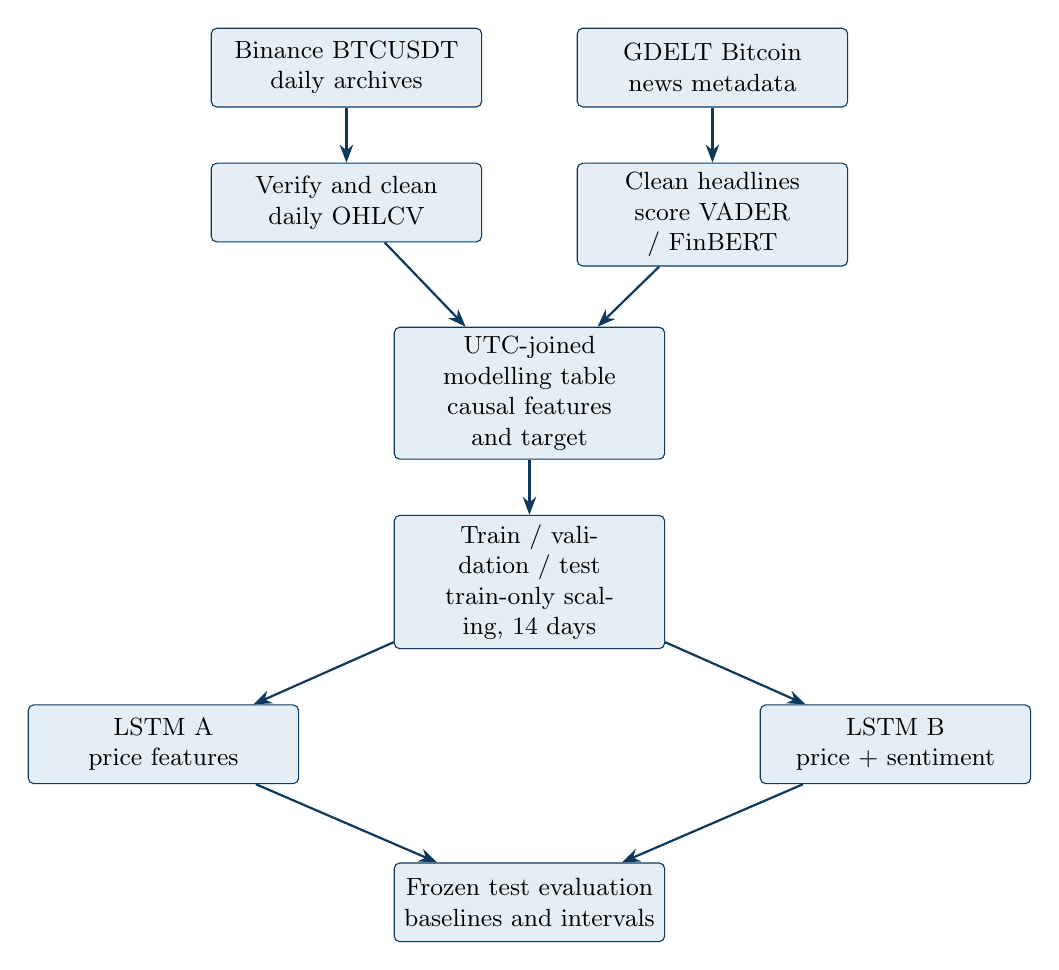
\begin{tikzpicture}[font=\small, node distance=7mm and 12mm,
 box/.style={draw=uowblue,fill=softblue,rounded corners=2pt,align=center,text width=3.2cm,minimum height=1.0cm},
 arr/.style={-{Stealth[length=2.3mm]},thick,draw=uowblue}]
\node[box] (bin) {Binance BTCUSDT\\daily archives};
\node[box,right=of bin] (gd) {GDELT Bitcoin\\news metadata};
\node[box,below=of bin] (p) {Verify and clean\\daily OHLCV};
\node[box,below=of gd] (n) {Clean headlines\\score VADER / FinBERT};
\node[box,below=15mm of $(p)!0.5!(n)$] (join) {UTC-joined modelling table\\causal features and target};
\node[box,below=of join] (spl) {Train / validation / test\\train-only scaling, 14 days};
\node[box,below left=of spl] (a) {LSTM A\\price features};
\node[box,below right=of spl] (b) {LSTM B\\price + sentiment};
\node[box,below=15mm of $(a)!0.5!(b)$] (eval) {Frozen test evaluation\\baselines and intervals};
\draw[arr] (bin)--(p);\draw[arr] (gd)--(n);\draw[arr] (p)--(join);\draw[arr] (n)--(join);\draw[arr] (join)--(spl);\draw[arr] (spl)--(a);\draw[arr] (spl)--(b);\draw[arr] (a)--(eval);\draw[arr] (b)--(eval);
\end{tikzpicture}
\caption{The experimental pipeline, from raw archives to the frozen test evaluation.}\label{fig:pipeline}
\end{figure}

\subsection{Target and information cutoff}
Let $C_t$ denote the Binance daily close on UTC date $t$. The target is
\begin{equation}\label{eq:target}
y_t=\begin{cases}1,&C_{t+1}>C_t,\\0,&C_{t+1}\leq C_t.\end{cases}
\end{equation}
An input window ending on date $t$ contains features from $t-13$ to $t$. Its label uses the close on $t+1$, which never appears as an input. The prediction is treated as made at 23:59:59 UTC on day $t$, so that full-day market data and eligible news are available by then. This is a daily close-to-close convention and does not describe trading at that instant.

News requires more care. Each headline has a GDELT batch timestamp and, in some cases, a precise publication time. Its availability is defined as the later of the two. This can delay a headline by hours or days. The choice is deliberately conservative, because a story should not count as known merely because its stated date precedes the moment at which the archive recorded it. Headlines are then grouped by the UTC date on which they became available.

\subsection{Chronological split}
A random split would mix neighbouring market conditions across sets, so ordered dates were assigned instead. The first 30 days of price history are dropped to give the technical indicators a full look-back, and the final price day serves only as the label for the preceding day. Because each input requires 14 consecutive days, a further 13 training endpoints are unavailable. The result is 1,418 training, 273 validation and 334 test sequences.

\begin{table}[htbp]\centering
\caption{Chronological split (dates give the last input day $t$)}\label{tab:split}
\begin{tabular}{llllr}
\toprule
Partition & First endpoint & Last endpoint & Up labels & Samples\\\midrule
Training & 13 Feb 2021 & 31 Dec 2024 & 704 (49.65\%) & 1,418\\
Validation & 1 Jan 2025 & 30 Sep 2025 & 139 (50.92\%) & 273\\
Test & 1 Oct 2025 & 30 Aug 2026 & 162 (48.50\%) & 334\\
\bottomrule
\end{tabular}
\end{table}

No observations are shuffled, and the scalers never see validation or test values. A later window may look back into earlier dates, since those observations existed before the prediction was made. Using a later target or fitting preprocessing on the future would be a different matter, and neither occurs here. All models are scored on identical test dates.

\subsection{Comparisons and hypotheses}
The primary null hypothesis states that adding VADER sentiment does not improve out-of-sample direction accuracy relative to the matched price-only LSTM. It is measured as $\Delta_{B-A}=\mathrm{Acc}(B)-\mathrm{Acc}(A)$ on the ensemble predictions, with positive values favouring sentiment. A paired bootstrap with 2,000 resamples of the test days gives a 95\% interval \cite{efron1993}. Adjacent days are not independent, and the interval is therefore read as an approximate guide and not as a formal significance test. Approaches designed for comparing classifiers on a single test set exist \cite{dietterich1998}, but they assume exchangeable observations that time-ordered data do not provide.

Balanced accuracy, precision, recall, F1, confusion matrices and the spread across seeds are reported as well. The majority rule and a price-only XGBoost classifier serve as increasingly demanding references. A sentiment-enhanced XGBoost and the FinBERT models are secondary checks and do not replace the primary comparison.

\subsection{Checks beyond the single split}
A single test window is a thin basis for a conclusion, and two further analyses were therefore added after the main evaluation. Both reuse the settings frozen earlier.

The walk-forward evaluation divides 2023 to 2026 into eight consecutive periods of about six months, following the rolling-origin principle \cite{tashman2000}. For each period the models are retrained on all earlier data, the last 90 days of that history are held out for early stopping, and the new period is used for testing. The pooled test set contains 1,338 days. Intervals for $\Delta_{B-A}$ are computed with blocks of seven days, because neighbouring errors tend to be correlated \cite{kunsch1989}.

The lag analysis is descriptive. It asks whether the sentiment on day $t$ is associated with the price move on day $t+k$, for $k$ from $-5$ to $+5$. Negative $k$ means that sentiment follows the move, and positive $k$ that it precedes it. Association is measured by Spearman's rank correlation \cite{spearman1904}. Significance is assessed with a circular-shift permutation test, a simple form of surrogate-data testing \cite{theiler1992} that preserves the autocorrelation of both series. The analysis covers January 2021 to mid-June 2025, before the news gap, and does not use the test period.

\subsection{Interpretation rules}
Three rules governed the writing. An analysis is described as completed only when code or saved output exists for it. Correlations are not given a causal reading. And an apparent gain on a reused test set is treated as exploratory, particularly when many tasks and models were tried. The last rule applies to the three-day, seven-day and large-move extensions, which can suggest hypotheses but cannot establish a new primary result without a fresh evaluation period.

\section{Data Collection}
\label{ch:data}
\subsection{Sources and study period}
Two sources were used. Binance Data Vision supplies BTCUSDT spot candles, and the GDELT Global Knowledge Graph supplies timestamped Bitcoin headlines \cite{binancepublic,leetaru2013,gdeltdata}. The two are complementary. The Binance archive is complete, structured and available at daily resolution. GDELT has broad historical coverage, but its headlines are multilingual and their timestamps require interpretation.

The study period runs from 1 January 2021 to 31 August 2026, which is 2,069 UTC days. The project requirements specified an end date of May 2025. Because both sources contained data well beyond that date, the window was extended by about fifteen months. The additional history is useful, but it also means that the final end date differs from the original plan, a point returned to in Section~\ref{ch:governance}.

\subsection{Binance prices}
The price data consist of 68 monthly ZIP archives of one-day BTCUSDT candles, each accompanied by a SHA-256 checksum file. All 68 checksums matched. The files carry no header, so the code assigns column names, converts values to numeric types and expresses every time in UTC. It also handles a change in the archives. From 2025 Binance recorded timestamps in microseconds instead of milliseconds, and a parser that ignored this would date those days tens of thousands of years in the future.

The cleaned table contains 2,069 rows, one per day, with no duplicate and no missing dates. Checks for positive prices, consistent high and low values and non-negative volume rejected no records. Twenty-four days on which the close changed by at least 10\% were reviewed individually. They correspond to identifiable events, such as the 14.4\% fall on 19 May 2021 and the 14.1\% fall on 9 November 2022 during the collapse of FTX, and were retained. Removing genuine crashes would make the data easier to model and the results less representative.

\figurewide{btc_history.pdf}{BTCUSDT daily close over the study period. Shading marks the validation and test periods.}{fig:history}

A single exchange and trading pair cannot represent the whole market. BTCUSDT is quoted in Tether, and prices on other venues may diverge during periods of stress. This restricts the setting to which the conclusions apply but does not affect the comparison between the models.

\subsection{GDELT headlines}
GKG 2.1 records were retrieved through Google BigQuery. The query keeps any record whose headline contains ``bitcoin'' or ``btc'', irrespective of case. Two exports cover the period. The 2021--2023 export contains 279,049 records and was extracted on 4 October 2026, scanning approximately 223~GB within BigQuery's free tier. The 2024--August 2026 export contains 261,469 records and was supplied from the team's first collection round. In total there are 540,518 raw records.

The exact SQL used for the second export was not preserved. A close equivalent was therefore reconstructed and compared with the delivered file for one month. For January 2024 the reconstructed query returns 17,486 rows against 16,780 in the delivered file, about 4\% more, which suggests that the original filter was slightly narrower. Because the reconstruction is at present the only version of that query that can be executed, the 4\% gap is a measured difference and not an established cause. It is relevant later because it probably accounts for a step in headline volume at the join between the two files.

Each record carries a GDELT batch timestamp, a precise publication time where one exists, the headline, URL, source, a translation flag and the \code{V2Tone} descriptor \cite{gdelttone}. \code{V2Tone} contains seven values: tone, positive and negative scores, polarity, activity density, self or group density and word count. These are GDELT's own measures and were not combined with VADER's compound score.

\subsection{Cleaning the headlines}
The cleaning code decodes HTML character references (twice where titles are doubly encoded), normalises Unicode, collapses whitespace and removes tracking parameters from URLs. It then discards headlines shorter than ten characters, machine-translated sources, text that a language detector confidently labels as non-English, and records that do not mention Bitcoin as a whole word. Duplicates are removed last, first by canonical URL and then by same-day normalised headline. VADER is an English lexicon, so non-English coverage was sacrificed to keep the sentiment measure consistent. The cost is substantial, since a large share of the global discussion is excluded.

Two steps account for most of the reduction. Removing machine-translated sources eliminated 208,998 headlines, and same-day duplicates removed a further 73,169. Table~\ref{tab:newsdrops} lists every step by period. Same-day duplicates were removed because syndicated stories would otherwise be counted many times and inflate the article volume.

\begin{table}[htbp]\centering\small
\caption{Headline accounting by period. The 2024--2026 column is the full-period figure minus the 2021--2023 figure.}\label{tab:newsdrops}
\begin{tabularx}{\textwidth}{Xrrr}
\toprule
Step & 2021--2023 & 2024--2026 & Full period\\\midrule
Raw GDELT records & 279,049 & 261,469 & 540,518\\
Empty or very short headline & 29 & 20 & 49\\
Machine-translated source & 106,718 & 102,280 & 208,998\\
Detected non-English & 645 & 230 & 875\\
Not Bitcoin-relevant & 6,245 & 80 & 6,325\\
Duplicate canonical URL & 469 & 158 & 627\\
Same-day duplicate headline & 44,228 & 28,941 & 73,169\\\midrule
\textbf{Retained for scoring} & \textbf{120,715} & \textbf{129,760} & \textbf{250,475}\\
\bottomrule
\end{tabularx}
\end{table}

The retained headlines are unevenly distributed over time. Coverage is thinnest in 2022, with 26,569 headlines or roughly 73 per day, and richest in 2024, with 67,261.

\subsection{Availability of a headline}
A headline is treated as available at the later of its GDELT batch time and its precise publication time, and it belongs to the UTC date of that moment. The rule sacrifices some immediacy but prevents inadvertent look-ahead. About half of all records have no precise publication time. Among the retained 2021--2023 headlines, 822 have a publication time more than seven days earlier than the time at which GDELT recorded them. Assigning these to their publication dates would have given the models news before the archive could have shown it.

\subsection{Coverage gaps and the volume step}
The daily sentiment table has 2,069 rows. For 17 consecutive days, from 15 June to 1 July 2025, no usable headline survived the cleaning. A neutral score was not imputed for these days. The rows carry a zero article count, an empty mean and a no-news flag, and the model input layer replaces the empty mean with a numerical value only in combination with that flag.

\figurewide{sentiment_coverage.pdf}{Monthly retained headline volume and average VADER score. The dashed line marks the start of the second export, and the shaded block is the 17-day gap.}{fig:newsvolume}

A second feature is the volume step. The mean daily article count rises from about 204 in December 2023 to about 302 in January 2024, where the two exports meet. This appears more consistent with a change in collection rules than with a sudden increase in Bitcoin news. The models therefore use sentiment shares and a logarithmic article count in place of raw counts. This mitigates the discontinuity without removing it, because the selection effect lies in the headlines themselves.

Headlines also describe the coverage of publishers and of GDELT, not investors. An article count measures media availability and not attention, and it does not count independent opinions.

\subsection{Data products}
The clean price file, the daily VADER table, the daily FinBERT table and the modelling table are stored in \code{data/processed/}. Headline-level files and the raw GDELT exports are excluded from the shared repository, which limits its size and avoids redistributing publishers' text. After the warm-up rows and the unlabelled final day are removed, the modelling table has 2,038 rows from 31 January 2021 to 30 August 2026, with 1,013 up days and 1,025 not-up days. Fourteen-day windows leave 2,025 usable endpoints. Calendar days, table rows and windows are kept distinct throughout, so that sample sizes are not confused.

\section{Data Governance}
\label{ch:governance}
\subsection{Purpose}
A forecasting pipeline can produce a tidy accuracy table while concealing doubts about the data behind it. A changed headline filter or an unnoticed timestamp leak can look exactly like a real signal. Governance is the means by which these risks were controlled. The source of each file was recorded, its integrity was verified, and each transformation applied to it was documented. These practices correspond to the principles of findable, accessible, interoperable and reusable data \cite{wilkinson2016} and to current recommendations for reproducible machine-learning research \cite{pineau2021}.

The raw Binance archives, their checksum files and the raw GDELT exports are kept unmodified. Python scripts build every derived table from them, and the source register, data dictionary and quality reports in the repository describe each step.

\subsection{Provenance and integrity}
For prices, 68 monthly Binance archives were downloaded and each was compared with the publisher's SHA-256 checksum. All 68 matched. The cleaned table holds 2,069 unique days and passed the checks for chronological order, positive prices, high and low bounds and non-negative volume.

For news, two BigQuery exports cover 1 January 2021 to 31 August 2026. The 2021--2023 file has 279,049 rows and covers all 1,095 days. Its SQL, schemas, row counts and exclusion counts are on record. Both raw files were fingerprinted so that the exact bytes used can be confirmed (Table~\ref{tab:hashes}).

\begin{table}[htbp]\centering\small
\caption{SHA-256 fingerprints of the raw GDELT exports used for the final results}\label{tab:hashes}
\begin{tabularx}{\textwidth}{p{3.4cm}rX}
\toprule
File & Rows & SHA-256\\\midrule
2021--2023 export & 279,049 & \texttt{\tiny 2e29cd2a29b7b9be8189c890bb02f142af2061062a152df4759e0c3843b90cd4}\\
2024--Aug 2026 export & 261,469 & \texttt{\tiny 695e1b6c6062a33ac65e1219d06ca50708b5d1eae9574bea8c91d4ba263d0415}\\
\bottomrule
\end{tabularx}
\end{table}

A separate audit pass over the 2024--2026 file retained all 261,469 records with quality flags and, after removing 44,341 repeated stories, left 217,128. It served as a cross-check of the cleaning. No model uses it, and its counts are not comparable with the stricter cleaning in Table~\ref{tab:newsdrops}.

\subsection{Timestamps and leakage}
Leakage is the principal way in which a sentiment model can mislead its authors. If a headline is treated as known on its stated publication date although the archive recorded it days later, the model is given information from the future. The adopted rule assigns each headline to the later of its GDELT batch time and its valid publication time. In the 2021--2023 data, 822 retained headlines were published more than seven days before GDELT recorded them, and counting them at their earlier dates would have constituted leakage.

The modelling code also verifies the rule directly. It raises an error if any headline counted on day $t$ became available after 23:59:59 UTC on that day, and a unit test covers the check. The 17-day gap in June 2025 is retained as missing and not filled, and the model observes it through an explicit flag.

These timing rules are controls against leakage, and no claim is made that they influence accuracy. Whether finer timing would improve prediction is a separate question, taken up in Section~\ref{ch:discussion}.

\subsection{Sharing, licensing and ethics}
All inputs are public market data or news metadata. No private accounts, trading histories or social-media profiles were collected. Binance publishes the price archive under its data terms \cite{binanceterms}, and GDELT may be used with citation \cite{gdeltterms}. The text of headlines nevertheless belongs to the publishers. For this reason the repository contains daily aggregates only, and neither the raw exports nor the headline-level tables are redistributed. The exported files used by the web interface go further: they contain no headline text and no article links, and the export script refuses to write either.

A review of the 234-file working tree on 15 October 2026 searched for hard-coded passwords, API keys, tokens, private keys, credential files and headline exports, and found none. The review covered the files as they stand and did not include the Git history. The pipeline uses no credentials at all, since every input is a public download.

It would also be inappropriate to present a near-chance classifier as investment advice. The results are an academic evaluation on historical data, and the interface states this on every page.

\subsection{Limits of the record}
Two gaps remain in the record, and both are small. The exact query behind the 2024--2026 export was not saved, so it was reproduced as closely as possible and the difference was measured (Section~\ref{ch:data}). The end date of 31 August 2026 also extends the original requirement of May 2025 because both sources supported it. Neither affects the comparison between models, since every model sees the same data, but both are relevant when reading the counts.

\section{Model Preparation}
\label{ch:preparation}
\subsection{Definition of the predictors}
The proposal referred to the trained predictors as agents. In this project the term denotes a classifier only. It accepts a window of market and news features and returns the probability that the following day closes higher. It does not browse the web, place orders or act autonomously. Preparation consists of converting raw data into comparable inputs, fixing the target and window, handling missing values and fitting scalers on the correct rows. A network cannot recover information that the pipeline never provided.

\subsection{Price indicators}
Standard indicators are derived from the current and earlier days only. They comprise the simple and logarithmic daily return and the ratios of the close to its 7-day and 30-day moving averages. Further indicators are 7-day and 14-day momentum, a 14-day relative strength index, 14-day volatility, the daily high-to-low range and a volume ratio. With $C_t$ denoting the close on day $t$,
\begin{align}
r_t &= \frac{C_t-C_{t-1}}{C_{t-1}}, &
\ell_t &= \log\left(\frac{C_t}{C_{t-1}}\right),\\
\operatorname{SMA}_{7,t}&=\frac{1}{7}\sum_{j=0}^{6}C_{t-j}, &
q_{7,t}&=\frac{C_t}{\operatorname{SMA}_{7,t}}.
\end{align}
No quantity on day $t$ uses a later day, and a unit test confirms this by altering future prices and checking that earlier features are unchanged.

Raw price levels and raw moving averages were excluded from the final inputs. The Bitcoin close ranged from about \$15{,}800 in November 2022 to about \$124{,}700 in October 2025. A scaler fitted on 2021--2024 would therefore encounter 2026 prices outside anything it had seen. Ratios and returns do not remove every shift, but they depend far less on the dollar level.

\begin{table}[htbp]\centering\small
\caption{The eleven price features used by Model A and reused unchanged by Model B}\label{tab:pricefeatures}
\begin{tabularx}{\textwidth}{p{4.4cm}X}
\toprule
Input & Construction\\\midrule
\code{return_1d} & Close-to-close simple return\\
\code{log_return_1d} & Logarithmic daily return\\
\code{close_over_sma_7} & Close divided by the 7-day moving average\\
\code{close_over_sma_30} & Close divided by the 30-day moving average\\
\code{momentum_7} & Relative price change over seven days\\
\code{momentum_14} & Relative price change over fourteen days\\
\code{rsi_14} & 14-day relative strength index\\
\code{volatility_14} & 14-day standard deviation of returns\\
\code{hl_range_pct} & Daily high-to-low range divided by the close\\
\code{volume_ratio_7} & Volume divided by its 7-day average\\
\code{log_volume} & Natural logarithm of daily base-asset volume\\
\bottomrule
\end{tabularx}
\end{table}

\subsection{Headline scoring and daily aggregation}
Each retained headline receives a VADER compound score. A score of at least $0.05$ is classed as positive and a score of at most $-0.05$ as negative, with values in between classed as neutral \cite{hutto2014}. The pipeline then summarises each UTC date by the mean score, the positive and negative counts, the number of eligible articles and the number of distinct sources. The LSTM never observes the headline text, only these daily summaries.

\begin{table}[htbp]\centering\small
\caption{The five additional inputs supplied to Model B}\label{tab:sentfeatures}
\begin{tabularx}{\textwidth}{p{4.5cm}X}
\toprule
Feature & Meaning\\\midrule
\code{vader_mean} & Mean compound score of day-$t$ articles\\
\code{vader_pos_share} & Positive articles divided by all articles, zero when there are none\\
\code{vader_neg_share} & Negative articles divided by all articles, zero when there are none\\
\code{log_article_count} & $\log(1+N_t)$, which reduces the effect of large volume swings\\
\code{no_news_flag} & One when no eligible article exists that day, otherwise zero\\
\bottomrule
\end{tabularx}
\end{table}

The aggregation involves considerable compression. A breaking regulatory story and a routine price summary carry equal weight in a daily mean. An article published at 23:55 is treated like one published at 00:05, although the former has almost no time left to influence the next close. Shares are less sensitive than raw counts to the volume step described in Section~\ref{ch:data}, but they do not remove it.

\subsection{FinBERT substitution}
The secondary pipeline scores the same 250,475 headlines with \code{ProsusAI/finbert}. Each headline receives positive, neutral and negative probabilities, and the daily features mirror the VADER ones: a mean score, positive and negative shares, the logarithmic article count and the no-news flag. Only the sentiment representation changes. The corpus, dates and target are identical.

The two scorers differ considerably. They assign the same label to 49.9\% of headlines, their headline-level scores correlate at 0.389, and their daily means correlate at 0.702. The two therefore measure related but distinct quantities. Without a human-labelled sample and a link to later returns, it is not possible to say which is closer to the truth.

\subsection{Alignment and missing days}
Each daily sentiment row is joined to the price row for the same UTC date, and the label is taken from the following day. A window ending at $t$ contains days $t-13$ to $t$ and never $t+1$. The code requires dates to be consecutive before any window is built, and no-news days remain in the series. This matters for a sequence model: if a missing week were dropped, the network would treat days that are seven days apart as neighbours.

A no-news day carries the binary flag and a neutral numerical default for the mean score. The default does not restore the missing information. Its function is to allow the flag to indicate that the value is a placeholder.

\subsection{Scaling and input shapes}
Each non-binary feature $j$ is standardised using the training mean and standard deviation:
\begin{equation}
z_{t,j}=\frac{x_{t,j}-\mu^{\mathrm{train}}_j}{\sigma^{\mathrm{train}}_j}.
\end{equation}
Validation and test rows reuse the stored values, and the no-news flag is passed through unscaled. A unit test confirms that changing validation or test values leaves the scaler unchanged.

Model A takes tensors of shape $[n,14,11]$ and Model B tensors of shape $[n,14,16]$, with $n$ equal to 1,418, 273 and 334 for training, validation and test respectively. Adjacent windows share thirteen of their fourteen days, so the training set contains considerably less independent evidence than 1,418 might suggest.

\subsection{Open design questions}
Some design choices merit caution. A 14-day look-back may be too short to capture medium-term effects, same-day averaging may blur the timing of a market reaction, and treating a 0.01\% rise identically to a 10\% rise discards information. All three were retained as specified, because changing them after observing test accuracy would have defeated the purpose of fixing the experiment in advance.

\section{Model Training}
\label{ch:training}
\subsection{Objective and models}
Each model outputs a probability $\hat p_t=P(y_t=1\mid X_t)$, and a rise is predicted when $\hat p_t\geq0.5$. The threshold was fixed before any evaluation and was never tuned. Training minimises binary cross-entropy, which penalises a confident wrong answer more heavily than a hesitant one.

Model A is a price-only LSTM. Model B has the same structure with the daily VADER features added, and the FinBERT version of Model B replaces the sentiment block and nothing else. XGBoost provides a tabular comparison, and the naive baseline predicts the training majority class on every day. The networks were implemented in PyTorch \cite{paszke2019}, the tree models with XGBoost \cite{chen2016}, and the metrics, scaling and utilities with scikit-learn, NumPy and pandas \cite{pedregosa2011,harris2020,mckinney2010}.

\subsection{LSTM architecture}
The network is small by design. It has one LSTM layer with 32 hidden units, a dropout layer \cite{srivastava2014} and a linear output passed through a sigmoid. If $h_{14}$ is the final hidden state after the 14-step window, then
\begin{equation}
\hat p_t=\sigma(Wh_{14}+b), \qquad \sigma(u)=\frac{1}{1+e^{-u}}.
\end{equation}
A bidirectional or attention-based model might fit the training years more closely, but it would add capacity and tuning freedom to a sample of 1,418 overlapping windows. A model that can be explained was preferred.

Training uses the Adam optimiser \cite{kingma2015}, gradient clipping at a norm of 1.0 \cite{pascanu2013}, mini-batches of 64 and a weight decay of $10^{-4}$. The weights with the best validation loss are kept, and training stops after 15 epochs without improvement. One detail is easily misreported. With a single recurrent layer, the dropout argument of the LSTM module has no effect, so the 0.2 dropout comes entirely from the explicit layer applied to the final hidden state.

\subsection{Selection and freezing of settings}
Twelve LSTM configurations were compared (16, 32 or 64 hidden units, one or two layers, dropout 0.2 or 0.4), each with both models and three seeds, using validation loss only. The configuration with the lowest mean validation loss over Models A and B was chosen, so both share one final set-up. XGBoost was tuned separately over six settings using validation log loss. The choices were written to file before the test days were used.

\begin{table}[htbp]\centering\small
\caption{Frozen primary settings}\label{tab:hyperparams}
\begin{tabularx}{\textwidth}{p{4.1cm}X}
\toprule
Setting & Value\\\midrule
Input history & 14 UTC days\\
Recurrent layers / hidden units & 1 / 32\\
Dropout & 0.20 (explicit, on the final hidden state)\\
Optimiser / learning rate & Adam / 0.001\\
Weight decay & $10^{-4}$\\
Batch size / maximum epochs & 64 / 150\\
Early-stopping patience & 15 epochs\\
Gradient clipping & Maximum norm 1.0\\
Final seeds & 100 to 109 (ten runs)\\
Probability threshold & 0.50\\
XGBoost depth / learning rate & 3 / 0.10\\
XGBoost other controls & Up to 500 trees, early stopping after 30, row and column subsampling 0.8, minimum child weight 5, L2 penalty 5\\
\bottomrule
\end{tabularx}
\end{table}

The selected mean validation losses were 0.6897 for the LSTM and 0.6878 for XGBoost. Both lie just below $\ln 2 = 0.6931$, the loss of a model that always predicts 50\%. This was taken as an early indication that the features carry little signal, and the test results later agreed. The final LSTMs were retrained with ten seeds, and the ensemble prediction for each day is the arithmetic mean of the ten probabilities and not a vote. Reporting several seeds follows the recommendation that variance across random initialisations should be accounted for when models are compared \cite{bouthillier2021}.

\subsection{Baselines and controlled alternatives}
The naive rule is learned from the training labels alone. The training set contains 704 up days out of 1,418, so its majority class is ``not up'', and it predicts that class on every day. The rule is trivial, yet it answers an important question: whether additional modelling improves on the simplest rule fitted to the same data.

XGBoost receives the engineered features of the last day as a flat row and not a fourteen-step sequence, so it is not a clean ablation of the LSTM. Its purpose is to test whether recurrence is worthwhile. An XGBoost with VADER features is also reported as an additional comparison.

The FinBERT models use the same headlines and test dates and inherit the frozen settings. No re-tuning was performed for FinBERT. This keeps the substitution interpretable, although it also means that FinBERT did not receive its own best hyperparameters.

\subsection{Protecting the test set}
Validation days select the settings and stop training early, and the test days appear once, in the final comparison. The evaluation script refuses to run without a frozen configuration and refuses a second run unless an explicit force flag is supplied. The saved result records zero reruns of the main test.

This does not cover every case. The FinBERT, extension and walk-forward analyses reuse the same later period, and they are therefore reported as secondary results alongside the primary one and never in its place. Averaging ten seeds indicates the sensitivity to random initialisation. It does not provide ten independent tests of the underlying hypothesis, because all ten train on the same market history.

\subsection{Saved artefacts}
\begin{table}[htbp]\centering\small
\caption{Files linking training to the reported results}\label{tab:artifacts}
\begin{tabularx}{\textwidth}{p{7.8cm}X}
\toprule
File or folder & Purpose\\\midrule
\code{src/make_splits.py} & Dated splits, scalers and 14-day windows\\
\code{results/frozen_config.json} & Validation-selected settings and seed lists\\
\code{results/model_settings.json} & Final features, package versions, dates and data hashes\\
\code{models/*.pt} & Ten weight files for each LSTM variant\\
\code{results/test_predictions.csv} & The 334 test-day predictions of the primary models\\
\code{results/test_metrics_per_seed.csv} & Per-seed test metrics and confusion counts\\
\code{results/final_results.json} & Primary ensemble comparisons and intervals\\
\code{results/finbert_results.json} & FinBERT comparison\\
\code{results/extension_results.json} & Other horizons and large-move tasks\\
\code{results/walk_forward/} & Eight-period walk-forward results and predictions\\
\code{results/lag_analysis/} & Lag correlations, quintile and feature tables\\
\bottomrule
\end{tabularx}
\end{table}

The run recorded Python 3.13.15 with pinned versions of PyTorch, XGBoost, scikit-learn, NumPy and pandas, and the repository includes a \code{requirements.txt} and a step-by-step README. The stored predictions allow the analysis to be repeated from the processed data without retraining the networks.

\subsection{Limits of the training stage}
Fixed-window classifiers were trained on historical data. No continuously adapting system, reinforcement-learning agent, trading strategy or live predictor was built. The ARIMA, GRU, CNN-LSTM and multi-asset branches of the proposal were not completed, and nothing in this report should be read as covering them.

\section{Result Analysis}
\label{ch:results}
\subsection{Test sample and reporting conventions}
The primary test comprises 334 daily predictions, with last input days from 1 October 2025 to 30 August 2026. Of these days, 162 were followed by a rise and 172 were not, giving an up-share of 48.50\%. Every headline comparison uses the same days and outcomes.

Two kinds of figure are reported. The \emph{mean} is the average of a metric over ten separately trained seeds. The \emph{ensemble} value is computed after averaging the ten models' probabilities for each day. The two need not coincide. If individual models fall on opposite sides of 0.5, their average can fall on either side, so ensemble accuracy is not the mean of the seed accuracies. The majority rule is run once and has no seed spread.

\subsection{Main next-day results}
\begin{table}[htbp]\centering\small
\caption{Primary held-out results on the 334 common test days. Mean $\pm$ SD is across seeds; ensemble columns use averaged probabilities.}\label{tab:mainresults}
\begin{tabularx}{\textwidth}{Xrrrr}
\toprule
Model & Mean acc. (\%) & SD (pp) & Ensemble acc. (\%) & Ensemble bal. acc. (\%)\\\midrule
Training-majority rule & 51.50 & --- & 51.50 & 50.00\\
LSTM A, price only & 48.71 & 1.41 & 50.00 & 49.82\\
LSTM B, price + VADER & 47.84 & 0.97 & 48.50 & 48.30\\
XGBoost, price only & 47.69 & 2.26 & 49.40 & 49.24\\
XGBoost, price + VADER (extra) & 48.68 & 2.43 & 47.90 & 47.71\\
LSTM B, price + FinBERT (secondary) & 48.53 & 1.24 & 47.90 & 47.70\\
\bottomrule
\end{tabularx}
\end{table}

The answer to RQ1 is negative. Model A reached 50.00\% and Model B with VADER 48.50\%, whereas the majority rule, which makes no attempt to read the market, scored 51.50\%. This does not indicate that the networks failed to train, since they learned structure from the training years. That structure did not translate into more correct calls on the held-out days.

\figurewide{accuracy_comparison.pdf}{Ensemble test accuracy of the main and secondary models. The dashed line is 50\%, although the actual majority baseline reaches 51.50\%.}{fig:comparison}

Precision, recall and F1 complete the picture. The majority rule never predicts a rise, so its positive-class precision, recall and F1 are zero by the convention of the evaluation code. It nevertheless leads on accuracy because the test period contains slightly more not-up days. The LSTMs predict both classes, but the additional rises they identify are offset by false alarms.

\begin{table}[htbp]\centering\small
\caption{Positive-class metrics of the ensembles on the main test split}\label{tab:prf}
\begin{tabularx}{\textwidth}{Xrrrr}
\toprule
Model & Precision (\%) & Recall (\%) & F1 (\%) & Balanced acc. (\%)\\\midrule
Majority not-up & 0.00 & 0.00 & 0.00 & 50.00\\
LSTM A & 48.30 & 43.83 & 45.95 & 49.82\\
LSTM B / VADER & 46.53 & 41.36 & 43.79 & 48.30\\
XGBoost / price & 47.65 & 43.83 & 45.66 & 49.24\\
LSTM B / FinBERT & 45.83 & 40.74 & 43.14 & 47.70\\
\bottomrule
\end{tabularx}
\end{table}

\subsection{Predictions against outcomes over time}
A single accuracy figure conceals how a model behaves from week to week. Figure~\ref{fig:predicted} therefore follows the test period day by day. Panel (a) shows the actual price, with the calls of the price-only LSTM marked as right or wrong. The model was right on 167 days and wrong on 167. The wrong calls are scattered along the whole path, and nothing in the figure suggests that the model reads the trend.

Panel (b) compares predicted probabilities with the outcomes. The black line is the share of up days in the preceding seven. It varies between 0 and 1, because seven-day stretches in this period were sometimes entirely up or entirely down. The blue and orange lines are the seven-day averages of the predicted probability of a rise for Models A and B. They remain close to 0.5. For Model A the seven-day average lies between 0.45 and 0.66, and for Model B between 0.44 and 0.62, while single-day probabilities for Model A range from 0.42 to 0.75. The networks therefore do not follow the swings in the ground truth. It appears that they learned to stay near 50\%, which is what a model does when the features carry little signal and the loss rewards caution.

Panel (c) shows rolling 30-day accuracy. Model A moves between 36.7\% and 70.0\%, Model B (VADER) between 33.3\% and 63.3\%, and the majority rule between 33.3\% and 73.3\%. No model remains ahead of the others for long, and the lead changes every few weeks. This is consistent with a result that is close to chance and is shaped by whichever month happens to suit a particular model.

\begin{figure}[htbp]\centering
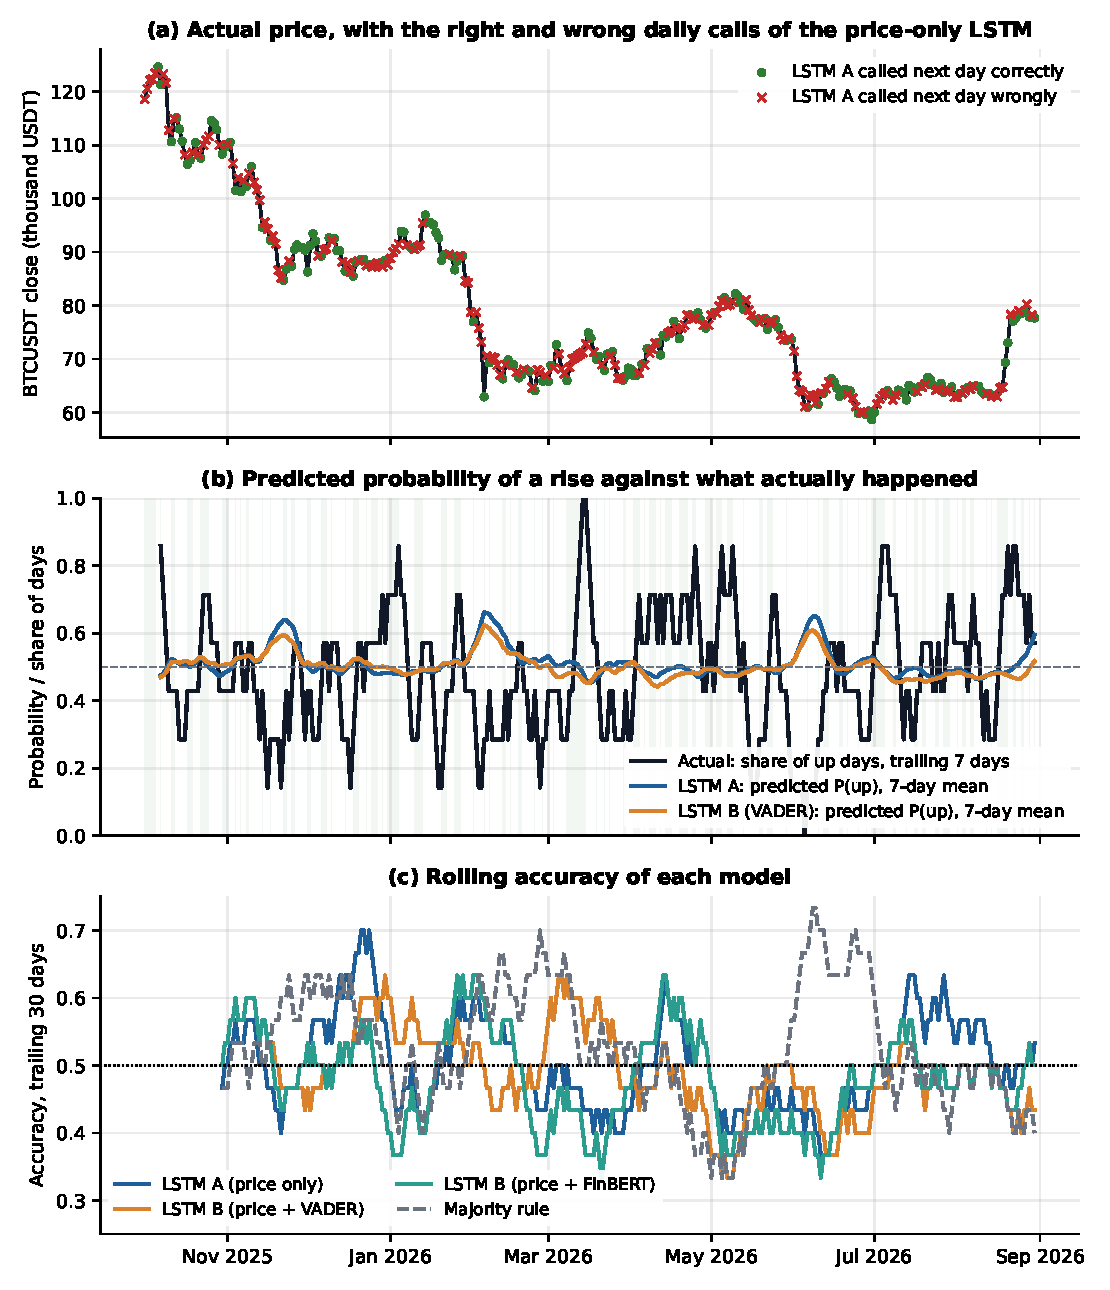
\includegraphics[width=0.93\textwidth]{figures/predicted_vs_actual.pdf}
\caption{Predictions against outcomes on the 334 test days. (a) Actual close, with right and wrong calls of LSTM A. (b) Trailing 7-day share of up days against the 7-day average predicted probability of a rise. (c) Trailing 30-day accuracy of each model.}\label{fig:predicted}
\end{figure}

\subsection{Confusion matrices}
The confusion matrix shows what the accuracy figure compresses. For the price-only LSTM, 96 not-up days and 71 up days were called correctly. A further 76 not-up days were wrongly called up, and 91 up days were missed. That gives 167 correct calls out of 334. The VADER model has 95 true negatives and 67 true positives, a total of 162 correct calls, five fewer than Model A.

\begin{table}[htbp]\centering
\caption{Ensemble confusion counts (rows give the actual outcome)}\label{tab:confusion}
\begin{tabular}{lrrrr}
\toprule
Model & TN & FP & FN & TP\\\midrule
Majority rule & 172 & 0 & 162 & 0\\
LSTM A & 96 & 76 & 91 & 71\\
LSTM B / VADER & 95 & 77 & 95 & 67\\
XGBoost price & 94 & 78 & 91 & 71\\
LSTM B / FinBERT & 94 & 78 & 96 & 66\\
\bottomrule
\end{tabular}
\end{table}

\figurewide{confusion_matrices.pdf}{Confusion matrices of the majority baseline and the two primary LSTM ensembles. Rows are the actual class and columns the predicted class.}{fig:cms}

Every model that predicts both directions faces the same trade-off. The additional correct rises must outweigh the additional false alarms on flat or falling days, and here they do not. Balanced accuracy remains close to 50\%, so the networks behave as weak classifiers.

\subsection{The sentiment effect and its uncertainty}
The primary sentiment effect is the difference between the matched ensembles,
\[
\Delta_{B-A}=0.48503-0.50000=-0.01497,
\]
or $-1.50$ percentage points. Balanced accuracy falls by 1.53 points. The paired bootstrap resamples the 334 days 2,000 times, always drawing the outcomes of Models A and B for the same days.

\begin{table}[htbp]\centering\small
\caption{Paired ensemble comparisons (Model B minus Model A)}\label{tab:delta}
\begin{tabularx}{\textwidth}{Xrrr}
\toprule
Difference & Point (pp) & 95\% interval (pp) & Excludes zero?\\\midrule
VADER B -- A, accuracy & $-1.50$ & $[-5.69,\ +2.40]$ & No\\
VADER B -- A, balanced accuracy & $-1.53$ & $[-5.71,\ +2.51]$ & No\\
FinBERT B -- A, accuracy & $-2.10$ & $[-5.40,\ +1.20]$ & No\\
FinBERT B -- VADER B, accuracy & $-0.60$ & $[-4.19,\ +3.00]$ & No\\
\bottomrule
\end{tabularx}
\end{table}

All four intervals include zero. The point estimates favour the simpler model, but the data cannot establish that sentiment is harmful, since a small gain and a moderate loss are both compatible with the intervals. The supportable conclusion is narrower: neither sentiment source showed a dependable benefit.

\subsection{From validation to test}
Model A's ensemble scored 57.14\% on validation and 50.00\% on test, a decrease of 7.14 points. Model B (VADER) fell from 52.75\% to 48.50\%, or 4.25 points, and XGBoost also lost ground. The models therefore learned relationships that did not carry fully into the later period, although a single split cannot indicate whether the cause was a changing market, selection optimism or both.

\figurewide{validation_vs_test.pdf}{Ensemble accuracy on validation and test days, from the saved evaluation files.}{fig:valtest}

Validation figures are flattered for a simple reason. The validation days helped to select the settings and the stopping epochs, so some optimism is built in even though the test days were never consulted. The 17-day news gap also lies in the validation period and not in the test period, which makes the two feature distributions differ.

\subsection{Probabilities clustered near the threshold}
With 334 days, the 95\% half-width for a guessing model is about 5.4 percentage points under independence. Serial dependence probably makes that figure optimistic. In either case, differences of one or two points are not persuasive.

The stored probabilities add a further observation. About 81.4\% of Model A's test predictions and 82.6\% of Model B's lie between 0.45 and 0.55. The networks are rarely confident, so a small change in a probability can alter a call. This describes the saved predictions and is not a new experiment.

\figurewide{probability_histograms.pdf}{Distribution of ensemble probabilities on the test days. Most lie close to the 0.5 threshold.}{fig:histprob}

\subsection{Walk-forward evaluation}
A single test window can flatter or penalise a model by chance, so the comparison was repeated eight times. Each period of about six months was tested by models retrained on all earlier data, using the same frozen settings and ten seeds. Together the periods cover 1,338 days from January 2023 to August 2026.

\begin{table}[htbp]\centering\small
\caption{Walk-forward results pooled over 1,338 test days. The guessing band is $50\% \pm 2.7$ points.}\label{tab:wfpooled}
\begin{tabularx}{\textwidth}{Xrrrr}
\toprule
Model & Mean acc. (\%) & SD (pp) & Ensemble acc. (\%) & Ensemble bal. acc. (\%)\\\midrule
Majority rule & 49.40 & --- & 49.40 & 50.00\\
XGBoost, price only & 48.86 & 0.48 & 47.53 & 47.75\\
LSTM A, price only & 51.19 & 0.96 & 51.42 & 51.60\\
LSTM B, price + VADER & 50.35 & 0.87 & 50.00 & 50.03\\
LSTM B, price + FinBERT & 50.89 & 0.70 & 52.17 & 52.26\\
\bottomrule
\end{tabularx}
\end{table}

The pooled picture agrees with the single split. Every model lies within about two points of 50\%, and the highest ensemble figure, 52.17\% for FinBERT, is still inside the guessing band. The sentiment effect also remains within the noise. VADER Model B minus Model A is $-1.42$ points (95\% interval $-4.04$ to $+1.05$), and FinBERT Model B minus Model A is $+0.75$ points ($-1.64$ to $+3.07$), using blocks of seven days to allow for correlated errors. Model B exceeded Model A in three of eight periods with VADER and in four of eight with FinBERT, which is about what chance would produce.

Table~\ref{tab:wffolds} shows how strongly the results vary between periods.

\begin{table}[htbp]\centering\small
\caption{Ensemble accuracy (\%) in each walk-forward period}\label{tab:wffolds}
\begin{tabularx}{\textwidth}{lrrrrrrr}
\toprule
Test period & Days & Up (\%) & Majority & XGBoost & LSTM A & B (VADER) & B (FinBERT)\\\midrule
Jan--Jun 2023 & 181 & 50.3 & 49.7 & 50.8 & 50.8 & 49.2 & 50.8\\
Jul--Dec 2023 & 184 & 50.5 & 49.5 & 46.7 & 49.5 & 53.3 & 55.4\\
Jan--Jun 2024 & 182 & 52.8 & 47.3 & 47.3 & 53.3 & 55.5 & 54.4\\
Jul--Dec 2024 & 184 & 52.2 & 47.8 & 47.8 & 53.3 & 47.8 & 52.2\\
Jan--Jun 2025 & 181 & 50.8 & 49.2 & 51.9 & 55.2 & 55.2 & 58.0\\
Jul--Dec 2025 & 184 & 49.5 & 50.5 & 47.8 & 53.3 & 47.8 & 50.0\\
Jan--Jun 2026 & 181 & 45.9 & 54.1 & 39.8 & 47.5 & 42.0 & 44.2\\
Jul--Aug 2026 & 61 & 57.4 & 42.6 & 49.2 & 42.6 & 47.5 & 52.5\\
\bottomrule
\end{tabularx}
\end{table}

Accuracy ranges from 39.8\% to 58.0\% across the cells, and it appears to follow the market's mix of up and down days more than it follows the model. January to June 2026 is the weakest full six-month period for every learned model, and only 45.9\% of its days closed higher. The majority rule, which predicts ``not up'' on every day, wins that period with 54.1\%. This is what pulled the main test result below 50\%, since the test window overlaps the last three periods. The strongest stretch, the first half of 2025, lies inside the validation window used to choose settings and is probably flattered. The two effects cannot be separated with these data.

\begin{figure}[htbp]\centering
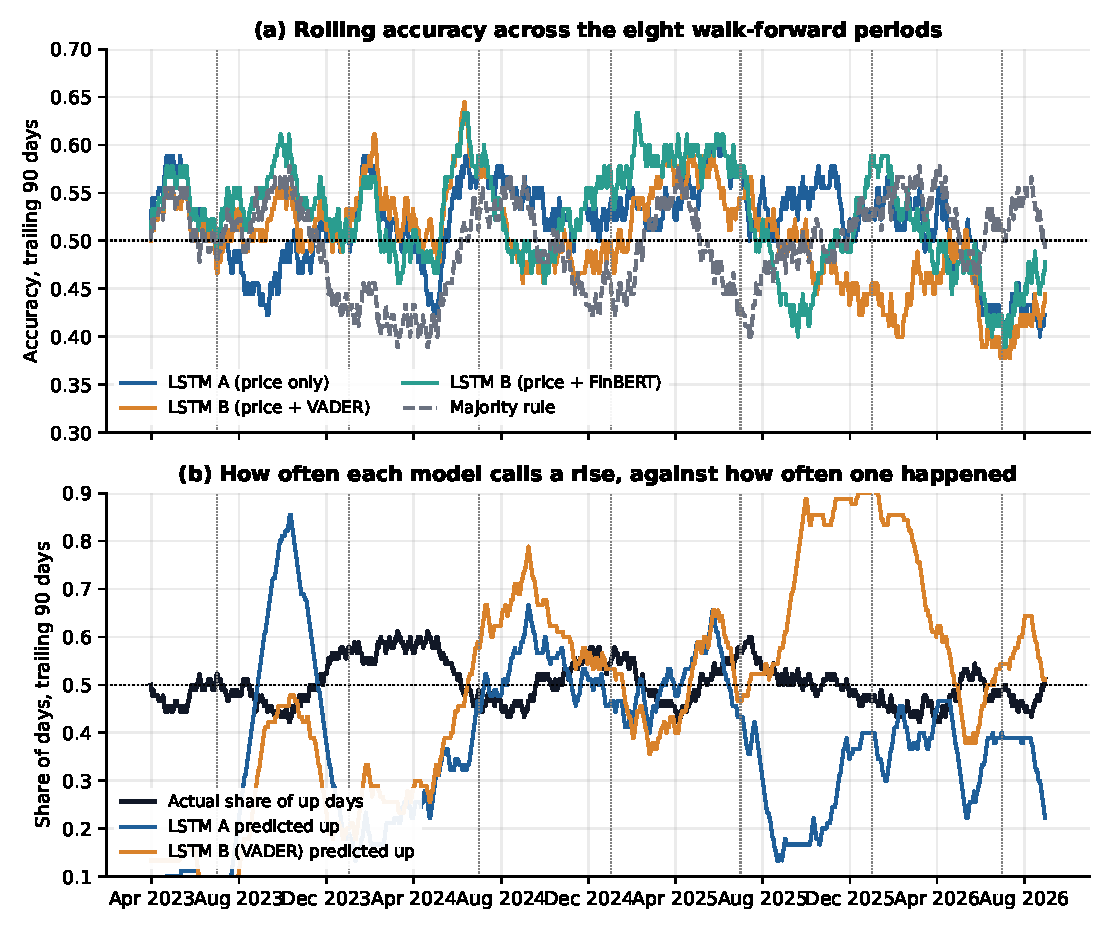
\includegraphics[width=0.93\textwidth]{figures/walkforward_rolling.pdf}
\caption{Walk-forward predictions over time, 2023 to 2026. (a) Rolling 90-day accuracy. (b) Share of days each model called a rise, against the share of days that actually rose. Dotted lines mark the start of each period.}\label{fig:wfroll}
\end{figure}

Figure~\ref{fig:wfroll} presents the curves over the full span. Rolling 90-day accuracy for LSTM A ranges from 40.0\% to 61.1\%, for B (VADER) from 37.8\% to 64.4\% and for B (FinBERT) from 38.9\% to 63.3\%. Panel (b) is more informative. The actual share of up days barely changes, from 42.2\% to 61.1\% in any 90-day window, whereas the models' share of rise calls ranges from 2.2\% to 85.6\% for Model A and from 3.3\% to 92.2\% for Model B. The models alternate between predicting almost every day up and almost every day down for months at a time, without tracking the real mix.

\figurewide{walkforward_folds.pdf}{Ensemble accuracy of each model in the eight walk-forward periods. The dotted line is 50\%.}{fig:wffolds}

\subsection{Does sentiment lead or follow price?}
The preceding results indicate that sentiment does not help. The lag analysis examines why. For each day it correlates the sentiment on day $t$ with the return on day $t+k$, for $k$ from $-5$ to $+5$. The sample is the 1,617 days from January 2021 to mid-June 2025, and the measure is Spearman's rank correlation \cite{spearman1904}.

\begin{figure}[htbp]\centering
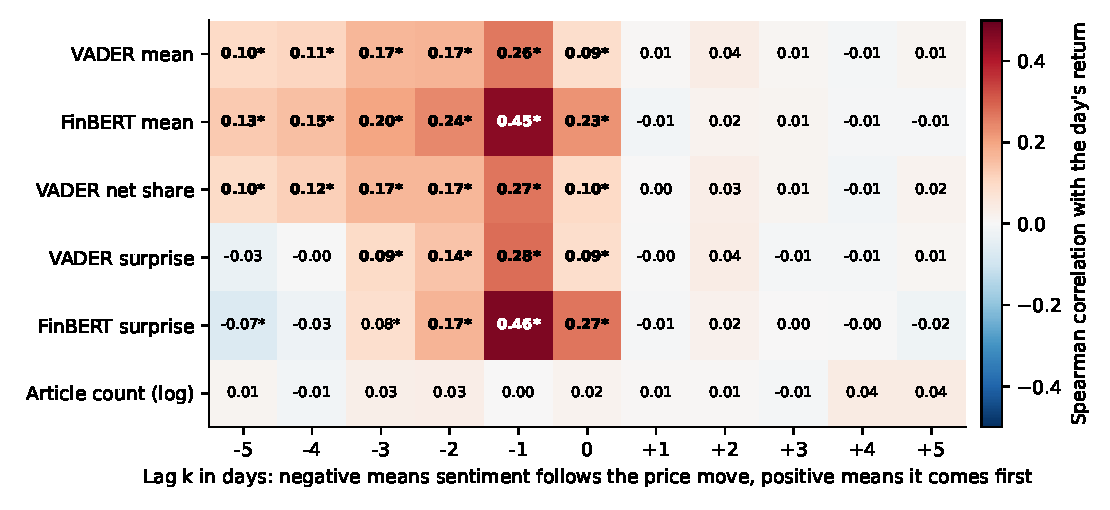
\includegraphics[width=0.95\textwidth]{figures/lag_heatmap.pdf}
\caption{Spearman correlation between day-$t$ sentiment and the return on day $t+k$. An asterisk marks a nominal $p<0.05$, and bold type marks significance after correction for 132 tests.}\label{fig:lag}
\end{figure}

The pattern in Figure~\ref{fig:lag} is asymmetric. Sentiment is associated with moves that have already happened. FinBERT's daily mean correlates 0.449 with the previous day's return ($k=-1$) and 0.225 with the same day's, whereas VADER's mean gives 0.262 and 0.089. Looking forward, the association disappears. At $k=+1$, the day the models predict, the correlations are $-0.012$ for FinBERT and $+0.005$ for VADER, with permutation $p$-values of 0.60 and 0.84.

Of the 132 tests, 32 reached $p<0.05$ against about 7 expected by chance, and 25 remained significant after a Bonferroni correction for the number of tests \cite{dunn1961}. All 25 have $k\leq0$. None of the tests with $k\geq1$ reached even $p<0.05$. Headlines on a given UTC day thus mostly describe the preceding day, so that by the time a score exists the price has already responded. The article count was likewise uninformative about the size of the next move.

Grouping days by sentiment level leads to the same conclusion. Across the five VADER groups the share of days followed by a rise ranges from 48.8\% to 51.7\%, and across the FinBERT groups from 47.7\% to 53.1\%, with no steady trend from pessimistic to optimistic days. The same-day association also varies from year to year (0.11 to 0.32 for FinBERT, $-0.02$ to $+0.12$ for VADER), which makes it a weak basis for a predictive model.

All 18 model inputs were also screened against the next day's direction. Five reached $p<0.05$ against 0.9 expected by chance, and three remained significant after correction: the daily return, the log return and the ratio of the close to its 7-day average. All three have negative sign. After an up day the next day is slightly more likely to be down, with an area under the ROC curve of about 0.55 once the sign is reversed \cite{fawcett2006}. No sentiment input came close. The reversal did not carry into the test period either, where every model remained near 48\%, so it should not be regarded as a stable signal.

\subsection{Monthly behaviour}
Month by month, Model A's test accuracy ranges from 45.2\% to 54.8\% and Model B's from 40.0\% to 61.3\%. With only 28 to 31 days per month, each figure carries a wide margin of error, and the plot is best read as a reminder that 50\% is an average of very uneven months.

\figurewide{monthly_test_accuracy.pdf}{Monthly test accuracy of the two LSTM ensembles. Each month has 28 to 31 days, so single-month differences carry little weight.}{fig:monthly}

\subsection{Summary}
Four findings stand out. The LSTMs do not beat the majority rule on the frozen test days. Adding sentiment from either VADER or FinBERT gives no dependable gain, on one split or across eight. The predicted probabilities remain near 50\%, and the calls drift between near-constant up and near-constant down over time. And sentiment correlates with past returns far more than with future ones, which offers a direct explanation of why it fails to forecast the next day.

\section{Benchmarking}
\label{ch:benchmark}
\subsection{Requirements of a fair benchmark}
Two published ``Bitcoin prediction'' figures can describe very different tasks, with other exchanges, date ranges, label definitions and test periods. Even within one project, a next-day up/down classifier should not be ranked beside a seven-day regression as if both measured the same quantity. The primary test is therefore treated as the single fixed yardstick: the same 334 dates, the same target, the same threshold and matched LSTM settings.

Absolute and incremental value are different matters as well. An accuracy of 50\% means little without a constant-class rule beside it. Here the majority rule scores 51.50\%, slightly above every primary learned ensemble, and this is the central benchmark finding.

\subsection{The majority-class rule}
The training set has 714 not-up days and 704 up days, so the rule always predicts ``not up''. On the test period 172 of 334 days were not-up, giving
\begin{equation}
\mathrm{Acc}_{\mathrm{majority}}=\frac{172}{334}=0.51497.
\end{equation}
The rule identifies no individual rise and has zero up-class recall. A claim that an LSTM is a useful direction classifier therefore has to explain why its additional errors are worthwhile, perhaps through better-calibrated probabilities \cite{guo2017}. The saved results provide no such justification.

A majority rule is not equivalent to a fair coin. A coin lands near 50\% on balanced labels, whereas the majority rule exploits class frequency and can exceed 50\% on a similar future period without any knowledge of the market. Both 50\% and the actual baseline are therefore reported, so that the gap to the neural models is not overstated.

\subsection{LSTM compared with XGBoost}
XGBoost operates on the engineered inputs as a flat row and has no recurrent state. Its price-only ensemble reached 49.40\% on the test days, with a seed average of 47.69\%. LSTM A's ensemble scored 50.00\%, only 0.60 points higher. This is far too small to claim an advantage for recurrence, and no paired interval was computed for this particular comparison. In the walk-forward test the ordering is clearer but still modest, with 51.4\% for LSTM A against 47.5\% for XGBoost over 1,338 days.

The additional XGBoost with VADER features scored 47.90\% as an ensemble. Its seed-average accuracy (48.68\%) was higher than that of the price-only version, but its ensemble accuracy was lower, so the two summaries disagreed. This is a reason not to exchange seed-average and ensemble figures.

\subsection{VADER compared with FinBERT}
A finance-trained language model appears a natural remedy for the weaknesses of VADER. The substitution did change the sentiment inputs, and the two scorers assign the same label to only half of the headlines. Yet the FinBERT LSTM ensemble reached 47.90\% on the test days, against 48.50\% for VADER and 50.00\% for price only. The paired difference to VADER was $-0.60$ points, with an interval from $-4.19$ to $+3.00$.

In the walk-forward test FinBERT was slightly ahead, with 52.17\% against 50.00\% for VADER and 51.42\% for price only. The interval for FinBERT minus price-only runs from $-1.64$ to $+3.07$ points, so this is not interpreted as a genuine gain. A stronger language model may classify a headline more accurately and still leave tomorrow's price equally unpredictable.

FinBERT inherited the frozen settings and was not tuned on its own, so these runs test the value of the substitution under shared conditions and do not establish an upper bound for FinBERT.

\subsection{Other horizons and large moves}
Three-day and seven-day direction were also examined, together with two tasks that train only on days with large moves. These were run after the primary set-up, use different labels and share the test period, so they are exploratory.

\begin{table}[htbp]\centering\small
\caption{Ensemble accuracy (\%) on the test days for the extension tasks. The 1\% and 2\% rows train only on days whose next-day move was at least that large, and score all test days.}\label{tab:extensions}
\begin{tabularx}{\textwidth}{Xrrrrr}
\toprule
Task & Test days & Majority & LSTM A & B (VADER) & B (FinBERT)\\\midrule
Next-day direction & 334 & 51.50 & 50.00 & 48.50 & 47.90\\
Three-day direction & 332 & 50.00 & 54.22 & 50.90 & 50.90\\
Seven-day direction & 328 & 45.43 & 51.22 & 46.65 & 47.26\\
Next day, trained on moves $\geq1\%$ & 334 & 48.50 & 50.60 & 49.10 & 48.80\\
Next day, trained on moves $\geq2\%$ & 334 & 48.50 & 47.90 & 48.50 & 49.70\\
\bottomrule
\end{tabularx}
\end{table}

\figurewide{horizon_extensions.pdf}{Ensemble accuracy at the three prediction horizons. These tasks were not pre-specified and are not directly comparable with the primary result.}{fig:extensions}

The three-day row attracts attention. LSTM A reached 54.22\%, while the sentiment models reached 50.90\%. This could indicate that price indicators carry some information at that horizon. When only every third day is scored, so that outcomes do not overlap, the figure falls to 52.25\% on 111 days. The seven-day price-only result of 51.22\% falls to 46.81\% on 47 non-overlapping weeks. A model without skill can deviate by $\pm9.3$ points at three days and $\pm14.3$ points at seven, so none of these differences is large enough to be relied on.

The large-move tasks changed little. Training on days with moves of at least 1\% (880 training windows) or 2\% (553 windows) left the LSTM ensembles between 47.9\% and 50.6\%, which is within the same noise. Scoring only the test days that turned out to be large appears more favourable in places: 53.57\% for LSTM A on the 196 days with a 1\% move, and 52.08\% for FinBERT on the 96 days with a 2\% move. These figures should not be relied upon. The size of tomorrow's move is unknown in advance, so such a subset cannot be selected in practice, and 96 days leaves a margin of about ten points.

Five tasks and several models on one period also constitute a multiple-testing problem. With so many scores, a few will exceed the baseline by chance alone \cite{harvey2016,bailey2014}.

\subsection{Interpreting the plateau}
It would be wrong to conclude that LSTMs predict Bitcoin at random in general. The narrower reading is that the signals provided here showed little ability to separate up days from the rest in this period. Several results point the same way. The majority rule edges out the learned models on the test days, balanced accuracies hover around 50\%, predicted probabilities cluster near the threshold, and sentiment does not help on one split or across eight. The lag analysis supplies a plausible reason, since the headlines trail the price.

Sample size matters as much as the ranking. With 334 days, a guessing model has a 95\% band of about $\pm5.4$ points, and overlapping windows and shifting regimes probably widen it. One model winning by 0.6 points is not an advantage in any statistical or economic sense.

\subsection{Published figures}
Several papers report strong sentiment gains \cite{huang2021,seabe2025,nezhad2026}. They are useful sources of ideas but not a leaderboard. A low percentage error on a continuous price is a different quantity from 50\% directional accuracy, and a model trained on minute-level social data and tested on a volatile stretch addresses a different problem from daily close-to-close classification. A fair external benchmark would require public data, the same label, the same decision time, the same held-out dates and preferably released predictions. In their absence, the internal baselines and fixed split offer firmer ground than numbers taken from other settings.

\subsection{Beyond accuracy}
Directional accuracy says nothing about monetary value. A correct call before a 0.1\% rise counts the same as one before a 10\% rise, and a small miss counts the same as a severe one. Assessing trading value requires a decision rule, a holding period, fees, slippage, risk limits and drawdown analysis, together with evidence that signals can be produced and acted upon at the cutoff. None of this was built, so the conclusion is limited to classification performance. On that measure no primary model beat the training-majority baseline on the fixed test days.

\section{Demonstration Interface}
\label{ch:demo}
\subsection{Purpose}
The preceding results are presented as tables and figures. To allow a reader to explore them interactively, a web interface was built that replays the saved predictions against the actual Bitcoin price. The interface does not retrain a model, retrieve live data or generate new predictions. Every quantity it displays is read from files that the pipeline has already produced.

\subsection{Functionality}
Figure~\ref{fig:demo} shows a full-page capture. A control panel at the top sets the period, the model and the prediction set.
\begin{itemize}
\item \textbf{Date selector.} Two date fields and five presets: the test period, the last three or six months, the last year, and all data.
\item \textbf{Model selector.} The majority rule, XGBoost, LSTM A, LSTM B with VADER and LSTM B with FinBERT.
\item \textbf{Prediction set.} The frozen test split (October 2025 to August 2026) or the walk-forward predictions, which cover January 2023 to August 2026.
\item \textbf{Price chart.} The daily close with one marker per day. A triangle pointing up or down gives the prediction for the next day. It is filled when the call was correct and hollow when it was wrong, so the chart does not depend on colour alone. Hovering reveals the close, the predicted direction and probability, the actual outcome and whether the call was right.
\item \textbf{Summary figures.} Accuracy for the chosen dates, shown beside the range that a guessing model would produce, the number of days, and the shares of predicted and actual rises.
\item \textbf{Sentiment chart.} Daily VADER or FinBERT scores for the same dates, with the no-news gap shaded and not hidden.
\item \textbf{Comparison table.} All five models scored on exactly the same days.
\end{itemize}
A banner on every page states that the output is experimental and not financial advice.

\begin{figure}[htbp]\centering
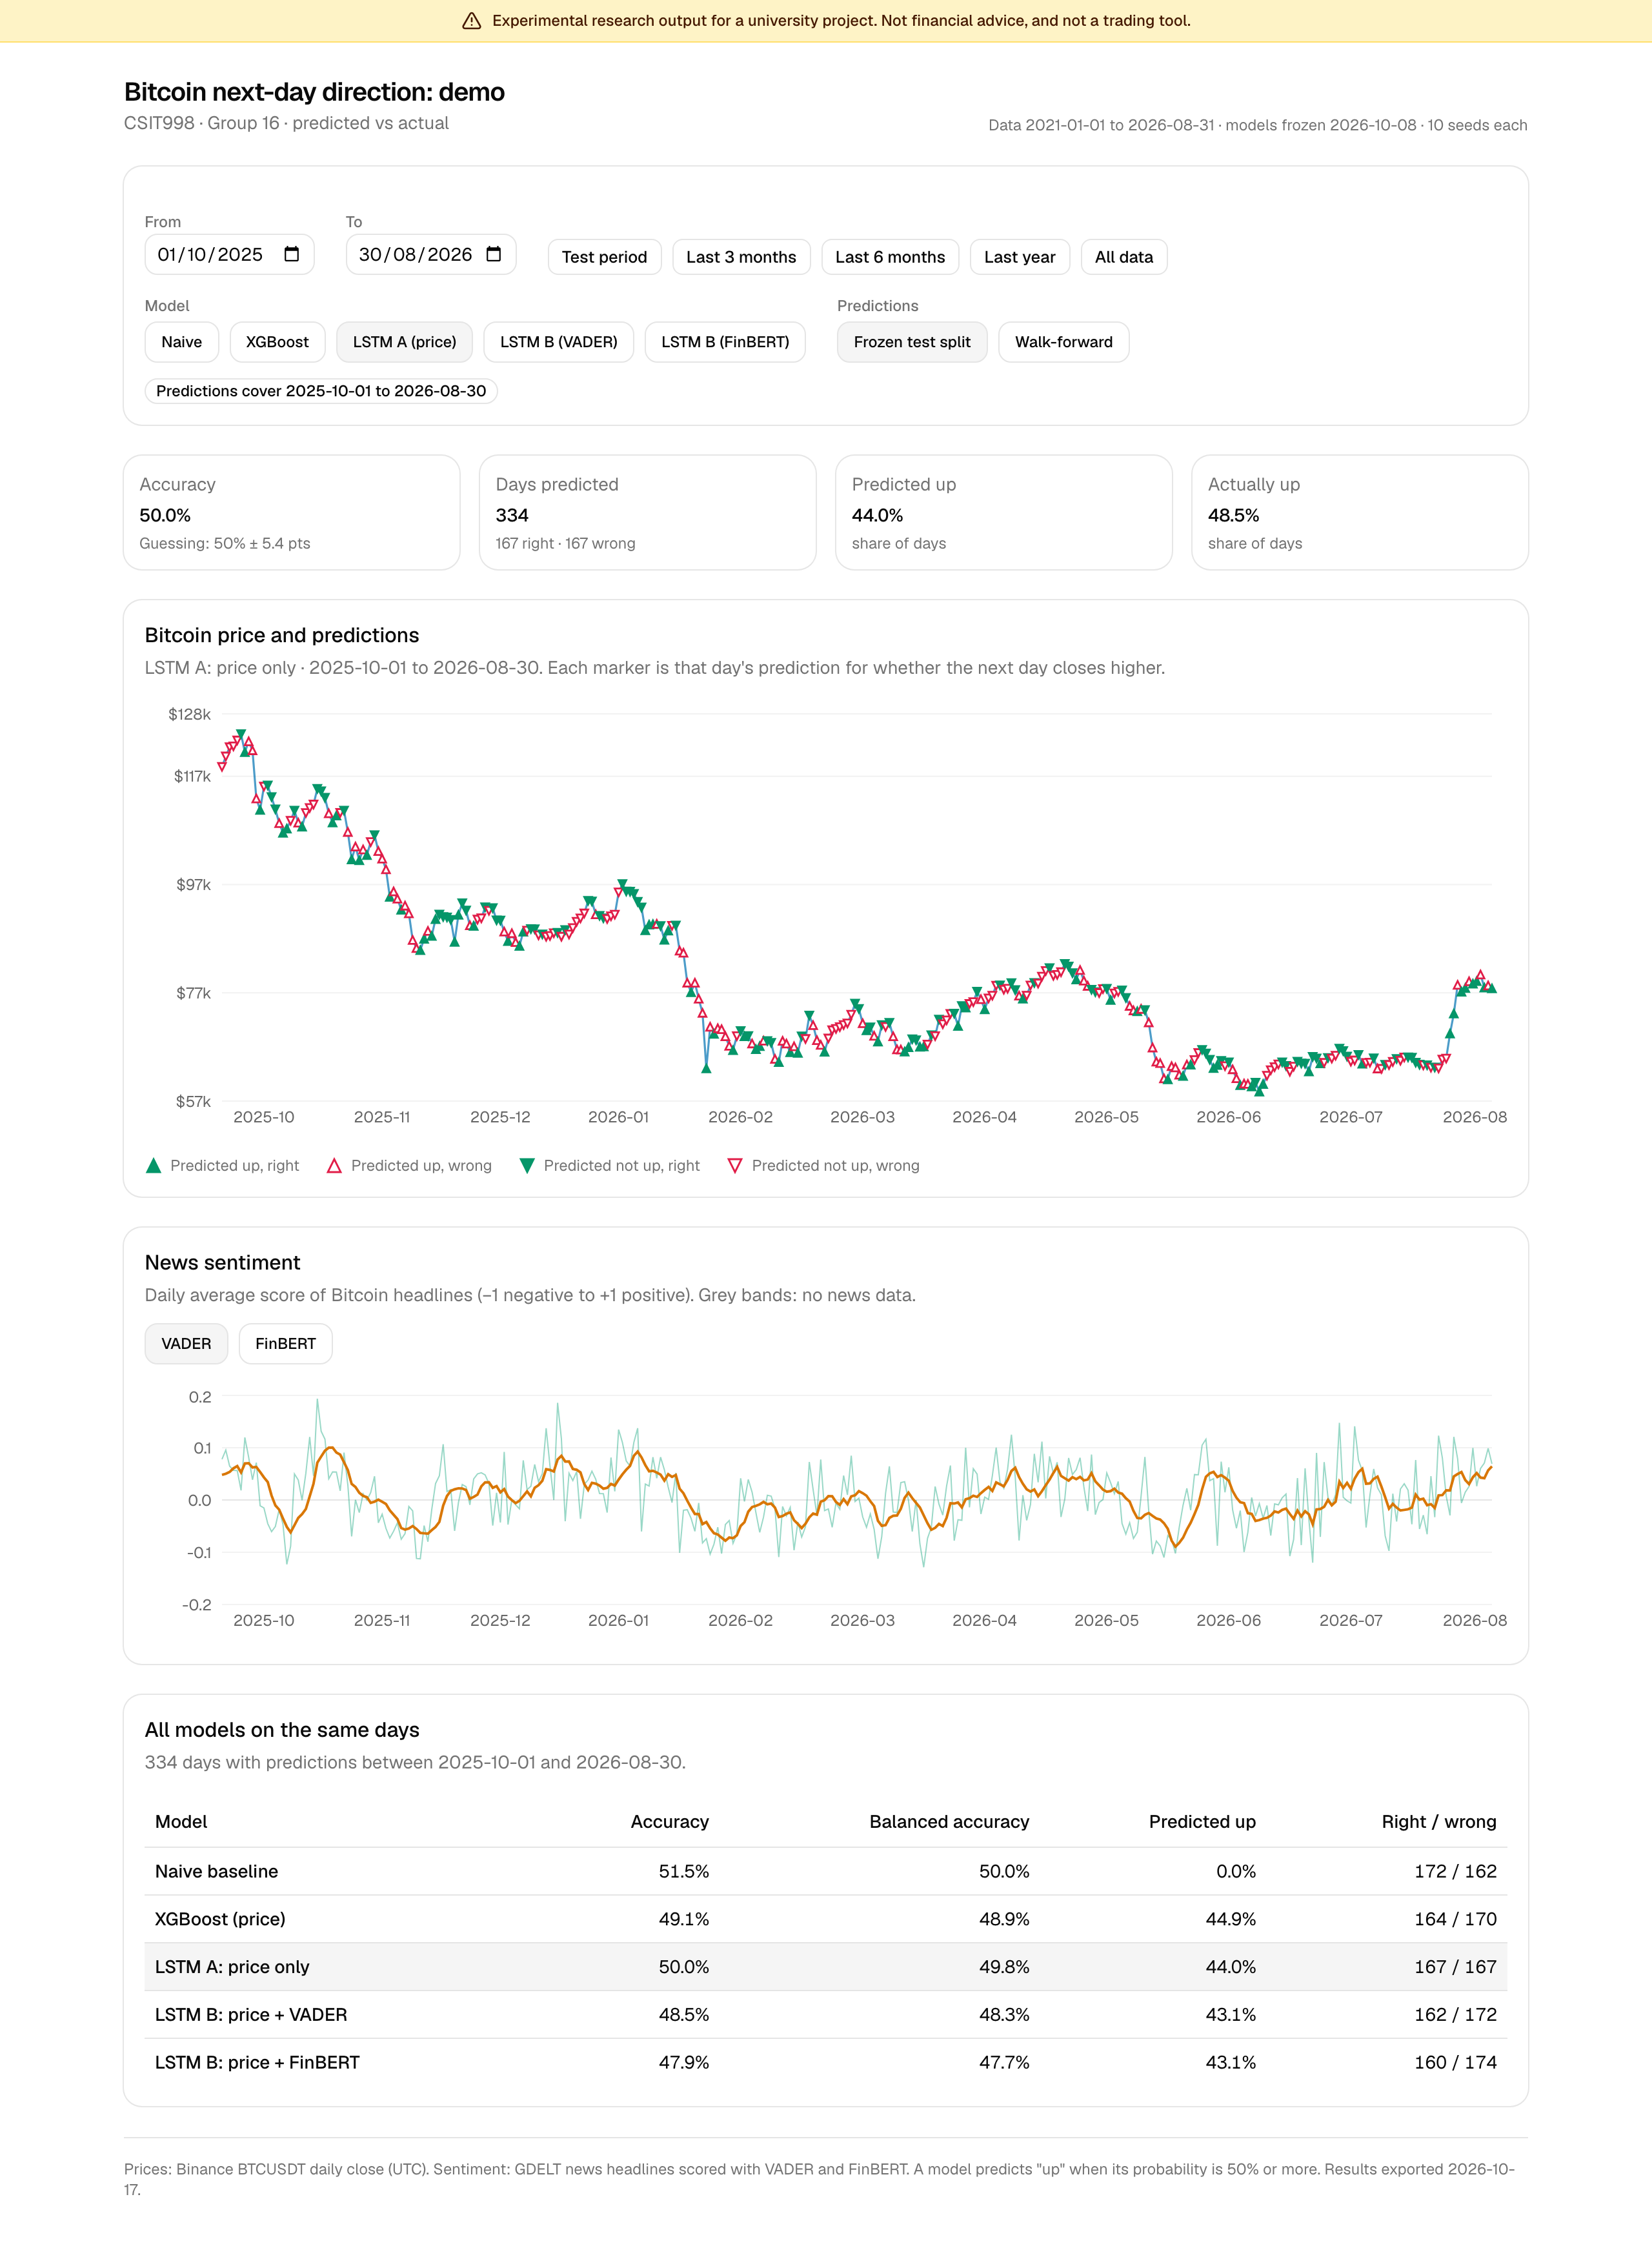
\includegraphics[height=0.78\textheight,keepaspectratio]{figures/demo_interface.png}
\caption{The demonstration interface, showing LSTM A on the frozen test period.}\label{fig:demo}
\end{figure}

\subsection{Implementation}
The interface is a Next.js application written in TypeScript, using Tailwind CSS, shadcn/ui components and the Recharts library, and exported as a static site. It has no server and no database. A Python script, \code{src/export_demo_data.py}, converts the saved results into three JSON files of about 460 KB in total. They hold the daily price and sentiment, each model's saved probability for every day, and a small metadata file. The site is built once from these files and can be hosted on any static service.

Two decisions follow from the governance work in Section~\ref{ch:governance}. The exported files contain only daily aggregates, with no headline text and no article links, and the export script refuses to write either. The page also computes its summary figures in the browser from the saved probabilities, using the same 0.5 threshold as the evaluation. A small test suite verifies this arithmetic together with the date presets.

To run the interface locally, the dependencies in the \code{web/} folder are installed and the development server is started. The README gives the exact commands.

\subsection{Limitations}
The interface replays history. It cannot produce a prediction for tomorrow, and this is deliberate. Given the results in Section~\ref{ch:results}, a live forecast would suggest skill that the evidence does not support. It also displays two prediction sets that were produced under different training schemes, and it labels them so that a viewer does not confuse them.

\section{Discussion}
\label{ch:discussion}
\subsection{Return to the research question}
The study began from a reasonable assumption: that market history together with news sentiment should describe the next day's Bitcoin direction better than market history alone. The experiment did not support it. Adding VADER reduced the price-only ensemble from 50.00\% to 48.50\% on the test days, and replacing it with FinBERT did not reverse the outcome. Across eight walk-forward periods the sentiment models stayed within about two points of the price-only model, in both directions. Because the paired interval on the single split extends from $-5.7$ to $+2.4$ points, it cannot be concluded that sentiment is harmful either. The defensible conclusion is that no incremental predictive value was found, which differs from showing that news is never informative.

The distinction deserves emphasis. A well-controlled negative result remains informative, because it shows which intuitions failed and under which conditions. The more productive question is therefore not how to raise the number but at which link of the chain the information is lost.

\subsection{Why accuracy remains close to 50\%}
\subsubsection{A difficult target}
The next day's close depends on events that do not exist at the cutoff, and traders can act on public information before a daily aggregate is computed. The efficient-market view makes weak predictability plausible \cite{fama1970}, although efficiency itself was not tested here. The class balance points the same way. The test period contains 48.50\% up days, so a model with almost no signal will remain near 50\% however it varies its calls, which is what the confusion matrices show.

\subsubsection{Sentiment follows price}
This is the clearest result obtained, and the lag analysis sharpens it. FinBERT's daily sentiment correlates 0.449 with the previous day's return and $-0.012$ with the next day's. For VADER the corresponding values are 0.262 and 0.005. None of the 60 forward-looking tests (all targets and measures with $k\geq1$) reached $p<0.05$, whereas 25 same-day or backward-looking tests remained significant after correction. The simplest reading is that a headline describes a move after it has occurred. GDELT also records stories some time after publication, and a daily bucket can place a reaction and its cause on the same date even when their order differs by hours.

The finding is a correlation and has the usual limits. Nonlinear, event-specific or very short-lived effects could lie behind it, and intraday timing was not examined. It nevertheless provides a concrete reason why a better sentiment classifier alone would not rescue the forecast. If the input describes an event that the price has already absorbed, a more accurate reading of it does not help.

\subsubsection{Daily averages obscure timing and meaning}
A day's mean sentiment collapses hundreds of headlines into one number. A short policy announcement is averaged with routine price summaries and paraphrased copies. A story at 00:05 and another at 23:55 fall in the same bucket, although one has a full day in which to matter and the other almost none. If a genuine effect lasts a few hours, a daily average would dilute it. Daily resolution was chosen for historical depth and reproducibility, and it may be one of the main reasons why sentiment did not help.

\subsubsection{Measurement noise and coverage}
VADER scores wording and FinBERT adds financial context, but neither was trained to estimate the effect of a headline on Bitcoin's next close. Both can be consistent as sentiment scorers and still address the wrong construct. Headlines were used in place of articles, and non-English and translated sources were removed, so a great deal of coverage is absent. The two GDELT exports used slightly different filters, which probably produced the step in headline volume in January 2024, and a 17-day gap lies in the validation period. Shares and a logarithmic count soften the volume problem without solving it.

\subsubsection{Limited independent training evidence}
The 1,418 training windows overlap so strongly that adjacent ones share thirteen days. They also cover one asset and a limited set of market regimes. Model B adds five inputs without adding a single new target day. If those inputs relate weakly or unstably to the next day's label, the additional dimensions make fitting less reliable even with dropout and early stopping. The test set contains 334 days, which allows a guessing model about $\pm5.4$ points of variation.

\subsubsection{Changing conditions}
Bitcoin's volatility, price level and news environment changed substantially between 2021 and 2026. Ratios reduce the dependence on scale but do not make the relationship stationary, and such instability is a recognised feature of financial series \cite{lo2004}. The walk-forward results show it directly. Period accuracy ranged from 39.8\% to 58.0\%, every learned model had its weakest full six-month period in the first half of 2026, and the decline of Model A from 57.14\% on validation to 50.00\% on test is consistent with the same pattern. It cannot be determined whether regime change, selection optimism or both were responsible. A single split provides one transition from past to future, and eight periods give a better impression of how fragile a signal is.

\subsubsection{A threshold that decides little}
The output is a probability, but headline accuracy applies a hard cut at 0.5. About four-fifths of the LSTM probabilities lie within 0.05 of it, so a small shift changes a call. Better calibration \cite{guo2017} or a rule that abstains when uncertain could help. Choosing a new cutoff that maximises accuracy on the same 334 days would not, since it would give an optimistic figure without stronger evidence. Any new threshold has to be derived from training and validation data and then confronted with fresh dates.

\begin{longtable}{p{3.1cm}p{5.6cm}p{5.0cm}}
\caption{Possible explanations for the plateau, the evidence available, and tests that would distinguish them}\label{tab:causes}\\
\toprule
Explanation & Evidence so far & Test that would help\\\midrule\endfirsthead
\toprule
Explanation & Evidence so far & Test that would help\\\midrule\endhead
Weak next-day signal & Classes near 50\%; no model beats the majority rule; walk-forward pooled accuracy 47.5\% to 52.2\% & A fresh period after August 2026\\
News follows price & Correlation 0.449 at $k=-1$, about 0 at $k=+1$ & First-seen timestamps and intraday windows\\
Over-aggregation & A daily mean ignores when a story appeared & Six-hour or hourly windows with a strict cutoff\\
Wrong construct & VADER and FinBERT agree on half of the labels, and neither helps & A human-labelled relevance sample; topic features\\
Coverage inconsistency & Volume step at January 2024; 17-day gap & One versioned query for both periods\\
Few independent samples & 1,418 overlapping windows, one asset & More assets or a longer history\\
Regime shifts & Period accuracy from 39.8\% to 58.0\%; validation-to-test drop of 7.1 points & Analysis by volatility regime\\
Threshold sensitivity & 81\% of probabilities within 0.45 to 0.55 & Validation-only calibration and abstention\\
Overfitting & Model B adds inputs without better scores & Feature ablations and a logistic baseline\\
\bottomrule
\end{longtable}

The right-hand column lists tests that were not carried out, and none of them should be counted as achieved.

\subsection{Would a larger network help?}
A near-chance result invites the response of attention layers, a deeper LSTM or a transformer. Such models can represent richer patterns, and earlier work shows specialised architectures performing well on some cryptocurrency tasks \cite{seabe2025,tiwari2025}. Capacity cannot, however, create information that is missing, late or unrelated to the target, and in a limited sample it increases the risk of fitting noise. A more cautious progression would start from the other end. A regularised logistic regression with price features and a single sentiment feature would show whether a sign-stable relationship exists at all, and only then would a larger model be warranted.

\subsection{Statistical interpretation and selective success}
The bootstrap interval for B minus A includes zero. This prevents a confident claim that VADER lowers accuracy, and it equally prevents treating a more favourable result on another seed, horizon or subset as success. Five tasks and several models were examined on related test days, so selective reporting is a genuine risk. Only a new period can confirm a hypothesis selected from these exploratory results \cite{bailey2014}.

The main bootstrap resamples single days. It preserves the pairing of the models but ignores serial dependence and therefore probably understates uncertainty. For the multi-day tasks and the pooled walk-forward results, blocks of days were resampled instead \cite{kunsch1989,politis1994}. Forecast accuracy can also be compared with tests designed for time series \cite{diebold1995}, which would be an appropriate refinement of the primary comparison.

\subsection{Relation to earlier work}
The gains reported by some sentiment-augmented studies were not reproduced. Several differences could account for this. Earlier work used social posts instead of headlines, domain-specific lexicons instead of VADER, finer horizons, price regression or different protocols \cite{huang2021,seabe2025,nezhad2026}. Their findings and ours can all be correct in their own settings. Comparing mechanisms and design is therefore more useful than comparing percentages, and a study reporting 95\% under a different label says nothing about whether the 50\% obtained here is poor.

\subsection{Limitations and practical meaning}
The analysis covers one pair on one exchange, a 2021 to 2026 history, daily binary direction, selected headlines and one final held-out period. The raw news files are not part of the shared code. Order-book depth, derivatives funding, macroeconomic releases and cross-asset flows were not used as features. The study also does not test whether any score would improve returns after costs. No execution simulation, position sizing or latency model was built, so no profitability claim follows. The artefacts are a research prototype that records the limits of its own evidence.

The positive outcome is methodological. A forecast cutoff was fixed, baselines were kept in view, a test period was frozen, the spread across seeds was stored, and interval estimates were reported that made an attractive result more cautious. These are real outcomes even though the predictor itself is not useful for decisions.

\section{Future Work}
\label{ch:future}
A list of every possible technique would be of little use. The next steps are therefore ranked by the gap in the evidence that each would close.

\subsection{Harmonising the news corpus and its timing}
The first requirement is methodological housekeeping. A single versioned BigQuery query should be run across the whole period, so that the 2021--2023 and 2024--2026 exports share one filter. This would show how much of the January 2024 volume step is a collection effect and how much reflects genuine change in coverage.

Timing is the second requirement. Where the metadata allow, the first-seen publication time should be retained and features computed over fixed windows that end before the cutoff. Stories that arrive late enough to affect the following close could then be distinguished from those that arrived in time to matter on the day. If the historical metadata cannot support this, the limitation should be stated and not circumvented by assumption.

\subsection{Testing on genuinely new dates}
Every result reported here comes from days that have now been examined. A clean confirmation requires a period after 31 August 2026, or a segment that was never used to choose extensions. Expanding-window backtests should continue, recording each fold's class balance, volatility, headline coverage and intervals. Log loss and the Brier score \cite{brier1950} would complement fixed-threshold accuracy. The aim is to learn how stable a signal is, and not to locate the one fold in which sentiment performs best.

\subsection{Modelling what a headline is about}
The lag analysis suggests that average daily tone mostly reflects the past. A more promising route is to model content. A classifier could separate regulation, exchange incidents, macroeconomic news, technical developments and routine price summaries, with source credibility, novelty and urgency as transparent inputs. A small, carefully sampled set of human labels would show whether VADER and FinBERT measure the intended quantity at all.

Timing deserves attention as well. Sentiment aggregated over the last 3, 6, 12 and 24 hours, built under the same no-look-ahead rule, would test whether temporal resolution was the missing element. A contextual encoder or attention layer is worth considering only after the inputs and timing have been validated.

\subsection{Simpler models and ablations}
Before adding LSTM capacity, a regularised logistic regression should be fitted and feature groups compared: price alone, price with mean sentiment, price with sentiment shares, and price with news volume. This would separate a weak sentiment score from a misleading volume artefact. The 14-day look-back should also be compared with 7, 30 and 60 days within a nested validation scheme. Other targets, such as three-day direction or large-move classification, deserve a proper test, and each new primary task requires its own fresh evaluation period.

\subsection{Regimes and economic value}
A fuller financial study would divide time into rising, falling, calm and turbulent regimes using only past or current information, and would ask whether sentiment helps mainly after unusual announcements. It could also test abstention, in which a model commits to a direction only when a validation-calibrated confidence is high \cite{guo2017}. This trades coverage for quality, so both the accuracy on retained days and the share of days skipped must be reported.

A trading backtest is appropriate only if a stable out-of-sample signal appears. It would require fees, spread, slippage, latency, turnover and drawdowns, and care would be needed to avoid backtest overfitting \cite{bailey2014}. A classifier with 52\% accuracy can still lose money, and the present evidence says nothing in either direction.

\subsection{Wider coverage}
Only one asset, one exchange and one news source were used. Ethereum, other venues and sources such as Reddit were outside the scope. Adding them would show whether the result is specific to Bitcoin headlines or reflects a broader weakness of daily sentiment. SHAP explanations would be informative once a model with real signal exists. Explaining a near-chance model has limited value.

\section{Conclusion}
\label{ch:conclusion}
This study examined whether news sentiment improves next-day Bitcoin direction forecasts. On the data available, it does not. A reproducible pipeline was built that joins 2,069 days of Binance BTCUSDT prices with 250,475 cleaned GDELT headlines. It applies explicit UTC availability rules, fits scalers on training days only, and compares matched models on fixed dates.

On the 334 held-out test days, a price-only LSTM ensemble classified 50.00\% of days correctly and the VADER version 48.50\%. A rule that always predicts ``not up'' scored 51.50\%. The 1.50-point difference between the two LSTMs came with a 95\% interval from $-5.69$ to $+2.40$ points, and FinBERT performed no better.

The comparison was then repeated across eight walk-forward periods covering 1,338 days. Pooled accuracy remained between 47.5\% and 52.2\% for every model. Adding sentiment shifted the price-only result by less than 1.5 points in either direction, and the intervals include zero.

The lag analysis offers the most useful clue about the reason. Sentiment correlates 0.45 with the previous day's return and approximately zero with the next day's, so the headlines trail the market. A signal that reports what has already happened cannot predict what follows. The predicted-versus-actual curves show the other aspect. On the test days the models' probabilities stay close to 0.5, and over several months they alternate between predicting almost every day up and almost every day down.

Several limits qualify these figures. The test set is small. The headlines come from two exports with slightly different filters, one news gap spans 17 days, and headlines were used instead of full articles. Intraday timing, other assets and trading returns were not examined. The extension and walk-forward analyses reuse the same later period, so they support the main result without replacing it.

The principal contribution is the method. A fixed cutoff, a strong trivial baseline, stored seeds, interval estimates and a frozen test set converted an attractive hypothesis into a cautious conclusion. A small web interface was also built that allows the predictions to be replayed against the actual price. A clear negative result obtained under these controls is a sounder basis for further work than an impressive accuracy figure that cannot be trusted.


\section*{AI Usage Disclosure}
\addcontentsline{toc}{section}{AI Usage Disclosure}

Generative AI (Claude and ChatGPT ) was used for  researching, grammar checking, formatting, and wording refinement. All project ideas, the experimental design, methodology, analysis and final content were formulated, reviewed, and verified by the project team.

\addcontentsline{toc}{section}{References}
% Reference list in the proposal-template format (numeric labels, in order of first citation).
% Generated from references.bib.
\begin{thebibliography}{63}
    \bibitem{sezer2020} Sezer, O. B., Gudelek, M. U., \& Ozbayoglu, A. M. (2020). Financial time series forecasting with deep learning: A systematic literature review: 2005--2019. Applied Soft Computing, 90, 106181. \url{https://doi.org/10.1016/j.asoc.2020.106181}
    \bibitem{fischer2018} Fischer, T., \& Krauss, C. (2018). Deep learning with long short-term memory networks for financial market predictions. European Journal of Operational Research, 270(2), 654--669. \url{https://doi.org/10.1016/j.ejor.2017.11.054}
    \bibitem{tetlock2007} Tetlock, P. C. (2007). Giving content to investor sentiment: the role of media in the stock market. The Journal of Finance, 62(3), 1139--1168. \url{https://doi.org/10.1111/j.1540-6261.2007.01232.x}
    \bibitem{kristoufek2013} Kristoufek, L. (2013). BitCoin meets Google Trends and Wikipedia: Quantifying the relationship between phenomena of the Internet era. Scientific Reports, 3, 3415. \url{https://doi.org/10.1038/srep03415}
    \bibitem{lo2004} Lo, A. W. (2004). The adaptive markets hypothesis: market efficiency from an evolutionary perspective. The Journal of Portfolio Management, 30(5), 15--29.
    \bibitem{cont2001} Cont, R. (2001). Empirical properties of asset returns: stylized facts and statistical issues. Quantitative Finance, 1(2), 223--236. \url{https://doi.org/10.1080/713665670}
    \bibitem{pineau2021} Pineau, J., et al. (2021). Improving reproducibility in machine learning research. Journal of Machine Learning Research, 22(164), 1--20.
    \bibitem{bouthillier2021} Bouthillier, X., et al. (2021). Accounting for variance in machine learning benchmarks. In Proceedings of Machine Learning and Systems, vol. 3.
    \bibitem{fama1970} Fama, E. F. (1970). Efficient Capital Markets: A Review of Theory and Empirical Work. The Journal of Finance, 25(2), 383--417. \url{https://doi.org/10.2307/2325486}
    \bibitem{urquhart2016} Urquhart, A. (2016). The inefficiency of Bitcoin. Economics Letters, 148, 80--82. \url{https://doi.org/10.1016/j.econlet.2016.09.019}
    \bibitem{nadarajah2017} Nadarajah, S., \& Chu, J. (2017). On the inefficiency of Bitcoin. Economics Letters, 150, 6--9.
    \bibitem{gu2020} Gu, S., Kelly, B., \& Xiu, D. (2020). Empirical asset pricing via machine learning. The Review of Financial Studies, 33(5), 2223--2273. \url{https://doi.org/10.1093/rfs/hhaa009}
    \bibitem{hochreiter1997} Hochreiter, S., \& Schmidhuber, J. (1997). Long Short-Term Memory. Neural Computation, 9(8), 1735--1780. \url{https://doi.org/10.1162/neco.1997.9.8.1735}
    \bibitem{gers2000} Gers, F. A., Schmidhuber, J., \& Cummins, F. (2000). Learning to forget: Continual prediction with LSTM. Neural Computation, 12(10), 2451--2471.
    \bibitem{mcnally2018} McNally, S., Roche, J., \& Caton, S. (2018). Predicting the price of Bitcoin using machine learning. In 26th Euromicro International Conference on Parallel, Distributed and Network-based Processing (pp. 339--343).
    \bibitem{jang2018} Jang, H., \& Lee, J. (2018). An empirical study on modeling and prediction of Bitcoin prices with Bayesian neural networks based on blockchain information. IEEE Access, 6, 5427--5437.
    \bibitem{huang2021} Huang, X., Zhang, W., Tang, X., Zhang, M., Surbiryala, J., Iosifidis, V., Liu, Z., \& Zhang, J. (2021). LSTM Based Sentiment Analysis for Cryptocurrency Prediction. arXiv preprint arXiv:2103.14804. \url{https://arxiv.org/abs/2103.14804}
    \bibitem{abraham2018} Abraham, J., Higdon, D., Nelson, J., \& Ibarra, J. (2018). Cryptocurrency price prediction using tweet volumes and sentiment analysis. SMU Data Science Review, 1(3). Article 1.
    \bibitem{girsang2023} Girsang, A. S., \& Stanley (2023). Cryptocurrency Price Prediction Based on Social Network Sentiment Analysis Using LSTM-GRU and FinBERT. IEEE Access. \url{https://doi.org/10.1109/ACCESS.2023.3324535}
    \bibitem{bollen2011} Bollen, J., Mao, H., \& Zeng, X. (2011). Twitter mood predicts the stock market. Journal of Computational Science, 2(1), 1--8. \url{https://doi.org/10.1016/j.jocs.2010.12.007}
    \bibitem{granger1969} Granger, C. W. J. (1969). Investigating causal relations by econometric models and cross-spectral methods. Econometrica, 37(3), 424--438. \url{https://doi.org/10.2307/1912791}
    \bibitem{loughran2011} Loughran, T., \& McDonald, B. (2011). When is a liability not a liability? Textual analysis, dictionaries, and 10-Ks. The Journal of Finance, 66(1), 35--65. \url{https://doi.org/10.1111/j.1540-6261.2010.01625.x}
    \bibitem{hutto2014} Hutto, C. J., \& Gilbert, E. (2014). VADER: A Parsimonious Rule-Based Model for Sentiment Analysis of Social Media Text. In Proceedings of the International AAAI Conference on Web and Social Media, vol. 8 (pp. 216--225). \url{https://doi.org/10.1609/icwsm.v8i1.14550}
    \bibitem{devlin2019} Devlin, J., Chang, M.-W., Lee, K., \& Toutanova, K. (2019). BERT: Pre-training of deep bidirectional transformers for language understanding. In Proceedings of the 2019 Conference of the North American Chapter of the Association for Computational Linguistics: Human Language Technologies (pp. 4171--4186).
    \bibitem{araci2019} Araci, D. (2019). FinBERT: Financial Sentiment Analysis with Pre-trained Language Models. arXiv preprint arXiv:1908.10063. \url{https://arxiv.org/abs/1908.10063}
    \bibitem{seabe2025} Seabe, P. L., Moutsinga, C. R. B., \& Pindza, E. (2025). Sentiment-driven cryptocurrency forecasting: analyzing LSTM, GRU, Bi-LSTM, and temporal attention model (TAM). Social Network Analysis and Mining, 15, 52. \url{https://doi.org/10.1007/s13278-025-01463-6}
    \bibitem{nezhad2026} Mohammadi Nezhad, M., Rouhani, S., Mohammadi, N., \& Shahedi, A. (2026). A unified GRU model for cryptocurrency price prediction and harsh price movement detection using enhanced sentiment analysis. Scientific Reports, 16, 16064. \url{https://doi.org/10.1038/s41598-026-46271-w}
    \bibitem{tiwari2025} Tiwari, D., Bhati, B. S., Nagpal, B., Alturki, N., \& Bayisenge, L. (2025). Attention-augmented hybrid CNN-LSTM model for social media sentiment analysis in cryptocurrency investment decision-making. Scientific Reports, 15, 33201. \url{https://doi.org/10.1038/s41598-025-18245-x}
    \bibitem{chen2016} Chen, T., \& Guestrin, C. (2016). XGBoost: A Scalable Tree Boosting System. In Proceedings of the 22nd ACM SIGKDD International Conference on Knowledge Discovery and Data Mining (pp. 785--794). \url{https://doi.org/10.1145/2939672.2939785}
    \bibitem{grinsztajn2022} Grinsztajn, L., Oyallon, E., \& Varoquaux, G. (2022). Why do tree-based models still outperform deep learning on typical tabular data? In Advances in Neural Information Processing Systems, Datasets and Benchmarks Track.
    \bibitem{brodersen2010} Brodersen, K. H., Ong, C. S., Stephan, K. E., \& Buhmann, J. M. (2010). The balanced accuracy and its posterior distribution. In 20th International Conference on Pattern Recognition (pp. 3121--3124).
    \bibitem{sokolova2009} Sokolova, M., \& Lapalme, G. (2009). A systematic analysis of performance measures for classification tasks. Information Processing and Management, 45(4), 427--437. \url{https://doi.org/10.1016/j.ipm.2009.03.002}
    \bibitem{tashman2000} Tashman, L. J. (2000). Out-of-sample tests of forecasting accuracy: an analysis and review. International Journal of Forecasting, 16(4), 437--450. \url{https://doi.org/10.1016/S0169-2070(00)00065-0}
    \bibitem{hyndman2021} Hyndman, R. J., \& Athanasopoulos, G. (2021). \emph{Forecasting: Principles and Practice} (3rd ed.). OTexts, Melbourne. \url{https://otexts.com/fpp3/}
    \bibitem{bergmeir2012} Bergmeir, C., \& Ben{\'i}tez, J. M. (2012). On the use of cross-validation for time series predictor evaluation. Information Sciences, 191, 192--213. \url{https://doi.org/10.1016/j.ins.2011.12.028}
    \bibitem{lopezdeprado2018} L{\'o}pez de Prado, M. (2018). \emph{Advances in Financial Machine Learning}. Wiley, Hoboken, NJ.
    \bibitem{bailey2014} Bailey, D. H., Borwein, J. M., L{\'o}pez de Prado, M., \& Zhu, Q. J. (2014). Pseudo-mathematics and financial charlatanism: The effects of backtest overfitting on out-of-sample performance. Notices of the American Mathematical Society, 61(5), 458--471.
    \bibitem{harvey2016} Harvey, C. R., Liu, Y., \& Zhu, H. (2016). \ldots and the cross-section of expected returns. The Review of Financial Studies, 29(1), 5--68. \url{https://doi.org/10.1093/rfs/hhv059}
    \bibitem{efron1993} Efron, B., \& Tibshirani, R. J. (1993). \emph{An Introduction to the Bootstrap}. Chapman and Hall, New York.
    \bibitem{dietterich1998} Dietterich, T. G. (1998). Approximate statistical tests for comparing supervised classification learning algorithms. Neural Computation, 10(7), 1895--1923. \url{https://doi.org/10.1162/089976698300017197}
    \bibitem{kunsch1989} K{\"u}nsch, H. R. (1989). The jackknife and the bootstrap for general stationary observations. The Annals of Statistics, 17(3), 1217--1241. \url{https://doi.org/10.1214/aos/1176347265}
    \bibitem{spearman1904} Spearman, C. (1904). The proof and measurement of association between two things. The American Journal of Psychology, 15(1), 72--101. \url{https://doi.org/10.2307/1412159}
    \bibitem{theiler1992} Theiler, J., Eubank, S., Longtin, A., Galdrikian, B., \& Farmer, J. D. (1992). Testing for nonlinearity in time series: the method of surrogate data. Physica D: Nonlinear Phenomena, 58(1--4), 77--94. \url{https://doi.org/10.1016/0167-2789(92)90102-S}
    \bibitem{binancepublic} Binance (2026). Binance Public Data: Spot Market Klines. Historical BTCUSDT 1-day OHLCV archives and checksum documentation; accessed 15 October 2026. \url{https://github.com/binance/binance-public-data}
    \bibitem{leetaru2013} Leetaru, K., \& Schrodt, P. A. (2013). GDELT: Global Data on Events, Location and Tone, 1979--2012. In ISA Annual Convention.
    \bibitem{gdeltdata} The GDELT Project (2026). GDELT Data: Querying, Analyzing and Downloading. Accessed 15 October 2026. \url{https://www.gdeltproject.org/data.html}
    \bibitem{gdelttone} The GDELT Project (2015). Global Knowledge Graph Data Format Codebook, Version 2.1. \url{https://data.gdeltproject.org/documentation/GDELT-Global_Knowledge_Graph_Codebook-V2.1.pdf}
    \bibitem{wilkinson2016} Wilkinson, M. D., et al. (2016). The FAIR Guiding Principles for scientific data management and stewardship. Scientific Data, 3, 160018. \url{https://doi.org/10.1038/sdata.2016.18}
    \bibitem{binanceterms} Binance (2026). Vision Dataset Terms and Conditions. Accessed 15 October 2026. \url{https://github.com/binance/binance-public-data/blob/master/TERMS_AND_CONDITIONS.md}
    \bibitem{gdeltterms} The GDELT Project (2026). GDELT Terms of Use and Citation. Accessed 15 October 2026. \url{https://www.gdeltproject.org/about.html}
    \bibitem{paszke2019} Paszke, A., et al. (2019). PyTorch: An imperative style, high-performance deep learning library. In Advances in Neural Information Processing Systems, vol. 32 (pp. 8024--8035).
    \bibitem{pedregosa2011} Pedregosa, F., et al. (2011). Scikit-learn: Machine learning in Python. Journal of Machine Learning Research, 12, 2825--2830.
    \bibitem{harris2020} Harris, C. R., et al. (2020). Array programming with NumPy. Nature, 585, 357--362. \url{https://doi.org/10.1038/s41586-020-2649-2}
    \bibitem{mckinney2010} McKinney, W. (2010). Data structures for statistical computing in Python. In Proceedings of the 9th Python in Science Conference.
    \bibitem{srivastava2014} Srivastava, N., Hinton, G., Krizhevsky, A., Sutskever, I., \& Salakhutdinov, R. (2014). Dropout: A simple way to prevent neural networks from overfitting. Journal of Machine Learning Research, 15(56), 1929--1958.
    \bibitem{kingma2015} Kingma, D. P., \& Ba, J. (2015). Adam: A method for stochastic optimization. In 3rd International Conference on Learning Representations. arXiv:1412.6980.
    \bibitem{pascanu2013} Pascanu, R., Mikolov, T., \& Bengio, Y. (2013). On the difficulty of training recurrent neural networks. In Proceedings of the 30th International Conference on Machine Learning, Proceedings of Machine Learning Research, vol. 28 (pp. 1310--1318).
    \bibitem{dunn1961} Dunn, O. J. (1961). Multiple comparisons among means. Journal of the American Statistical Association, 56(293), 52--64. \url{https://doi.org/10.1080/01621459.1961.10482090}
    \bibitem{fawcett2006} Fawcett, T. (2006). An introduction to ROC analysis. Pattern Recognition Letters, 27(8), 861--874. \url{https://doi.org/10.1016/j.patrec.2005.10.010}
    \bibitem{guo2017} Guo, C., Pleiss, G., Sun, Y., \& Weinberger, K. Q. (2017). On calibration of modern neural networks. In Proceedings of the 34th International Conference on Machine Learning, Proceedings of Machine Learning Research, vol. 70 (pp. 1321--1330).
    \bibitem{politis1994} Politis, D. N., \& Romano, J. P. (1994). The stationary bootstrap. Journal of the American Statistical Association, 89(428), 1303--1313. \url{https://doi.org/10.1080/01621459.1994.10476870}
    \bibitem{diebold1995} Diebold, F. X., \& Mariano, R. S. (1995). Comparing Predictive Accuracy. Journal of Business and Economic Statistics, 13(3), 253--263.
    \bibitem{brier1950} Brier, G. W. (1950). Verification of forecasts expressed in terms of probability. Monthly Weather Review, 78(1), 1--3.
\end{thebibliography}


\appendix
\section{Implementation and Reproduction}
\label{app:repro}
\subsection{Layout and execution order}
The repository contains \code{src/}, \code{tests/}, \code{data/}, \code{reports/}, \code{results/}, \code{models/}, \code{docs/}, \code{report/} and \code{web/} folders. Each Python stage reads the output of the preceding one. From the repository root, after installing the pinned packages listed in \code{requirements.txt}, the sequence is:

\begin{lstlisting}[basicstyle=\ttfamily\footnotesize,backgroundcolor=\color{codegray},breaklines=true,frame=single]
python -m src.prepare_price
python -m src.prepare_news
python -m src.build_sentiment
python -m src.build_modelling_table
python -m src.make_splits
python -m src.tune
python -m src.evaluate_final
# secondary analyses
python -m src.score_finbert
python -m src.build_finbert_features
python -m src.evaluate_finbert
python -m src.evaluate_extensions
python -m src.lag_analysis
python -m src.walk_forward
# figures, demo data and tests
python -m src.make_report_figures
python -m src.export_demo_data
pytest -q
# web interface
cd web && pnpm install && pnpm test && pnpm build
\end{lstlisting}

The main evaluator requires a frozen configuration and refuses a second run unless an explicit force flag is supplied. The extension, FinBERT and walk-forward scripts follow the same rule. These guards exist to prevent tuning against the test score.

\subsection{Data and result fingerprints}
The final results record SHA-256 fingerprints of the modelling table, the saved sequences and the processed price file:
\begin{lstlisting}[basicstyle=\ttfamily\footnotesize,backgroundcolor=\color{codegray},breaklines=true,frame=single]
modelling_table_v1.csv
c4d946539b93a237d902a6609fd32c63cdccba31dd70089b226140f078aae12b
sequences.npz
97df12e1a2c48c277ba17bebdaad06b7841ce012ade586321b2842abb13a123a
btcusdt_1d_clean.csv
ae28258b7e5bc319591dc3edc23240411765e6d2c0477bf358e6e089e4c8b36c
\end{lstlisting}
The fingerprints of the two raw GDELT exports appear in Table~\ref{tab:hashes}.

Model weights are stored in \code{models/}, one file per seed (100 to 109) and model variant, with names such as the following.
\begin{lstlisting}[basicstyle=\ttfamily\footnotesize,backgroundcolor=\color{codegray},breaklines=true,frame=single]
lstm_a_price_only_seed100.pt
\end{lstlisting} The results folder keeps the predictions and per-seed metrics, so that the evaluation figures can be redrawn without retraining.

\subsection{Levels of reproducibility}
Reproducibility can be stated at three levels. At the code level, the methods exist as executable files. At the processed-data level, a user can rerun the modelling from the saved features and outputs. At the source-data level, the original exports, matching queries and permission to use them are also required. The repository supports the first two. The raw GDELT files contain publishers' text and are not distributed. A rebuild from raw data therefore requires the two exports to be queried again (the 2021--2023 SQL is given in \code{docs/}) under their usage terms.

\section{Definitions}
\label{app:definitions}
\subsection{Market and article definitions}
The daily market record is the Binance one-day BTCUSDT candle in UTC, identified by its opening time. The simple return is $r_t=C_t/C_{t-1}-1$ and the target is $y_t=\mathbb{1}(C_{t+1}>C_t)$. When two consecutive closes are equal the target is 0. There is no separate class for an unchanged price.

A retained article is an eligible, deduplicated GDELT headline whose availability date falls on the given UTC day. The daily article count is the number of such records and not the number of stories published anywhere. Positive and negative shares divide the category counts by that retained count, and no-news days carry their own flag, so that a missing input is not read as a neutral mood.

\subsection{Classification metrics}
With the up class taken as positive,
\begin{align}
\mathrm{Accuracy} &= \frac{TP+TN}{TP+TN+FP+FN},\\
\mathrm{Precision} &= \frac{TP}{TP+FP},\qquad
\mathrm{Recall} = \frac{TP}{TP+FN},\\
\mathrm{Specificity} &= \frac{TN}{TN+FP},\qquad
\mathrm{BalancedAcc} = \frac{\mathrm{Recall}+\mathrm{Specificity}}{2},\\
F_1 &= \frac{2\,\mathrm{Precision}\,\mathrm{Recall}}{\mathrm{Precision}+\mathrm{Recall}}.
\end{align}
These measures are standard \cite{sokolova2009,brodersen2010}. A model that never predicts a rise has an undefined precision. The scikit-learn implementation sets it to zero, so that recall and F1 are also zero, which is why the majority rule can show 51.50\% accuracy together with zero F1. Log loss for probabilities $p_i$ is
\begin{equation}
L=-\frac{1}{n}\sum_{i=1}^{n}\left[y_i\log p_i+(1-y_i)\log(1-p_i)\right],
\end{equation}
and it uses the full probability, which makes it more sensitive to overconfidence than thresholded accuracy. The area under the ROC curve, used in the feature screening, equals the probability that a randomly chosen up day receives a higher feature value than a randomly chosen not-up day \cite{fawcett2006}.

\subsection{Uncertainty methods}
\textbf{Paired bootstrap (single split).} The script draws 334 test-day indices with replacement and computes each model's metric on the drawn days. It subtracts the Model A value from the Model B value and repeats the procedure 2,000 times with a fixed seed \cite{efron1993}. The 2.5th and 97.5th percentiles give the interval. Pairing keeps both models on identical resampled days.

\textbf{Block bootstrap (multi-day and walk-forward).} The same procedure resamples blocks of consecutive days \cite{kunsch1989}. The block length is seven days for the pooled walk-forward results and equal to the horizon for the multi-day tasks. Neighbouring days share outcomes or have correlated errors, so block resampling gives a more realistic interval. A stationary variant with random block lengths is also available \cite{politis1994}.

\textbf{Circular-shift permutation test (lag analysis).} For each sentiment measure and lag, one series is rotated by a random offset 5,000 times while the other remains fixed. This preserves the autocorrelation of both series and breaks any genuine association between them, in the manner of surrogate-data tests \cite{theiler1992}. The $p$-value is the proportion of rotations whose correlation is at least as large in magnitude as the observed one. With 132 tests the Bonferroni threshold is $0.05/132\approx0.00038$ \cite{dunn1961}.

\textbf{Guessing band.} For $n$ independent days, a model without skill has a 95\% accuracy band of $50\%\pm1.96\sqrt{0.25/n}$, which is $\pm5.4$ points for 334 days and $\pm2.7$ for 1,338. For $h$-day targets $n$ is divided by $h$, since overlapping outcomes carry less independent information.

\section{Requirements Traceability}
\label{app:trace}
\subsection{Requirements and supporting evidence}
The table maps the principal requirements of the September requirements draft to the evidence in the repository.

\begin{longtable}{p{2.5cm}p{4.0cm}p{7.0cm}}
\caption{Requirements and supporting evidence}\label{tab:trace}\\
\toprule
Requirement & Intent & Evidence\\\midrule\endfirsthead
\toprule
Requirement & Intent & Evidence\\\midrule\endhead
DR-01 & Daily BTC coverage & 68 Binance monthly archives; 2,069 verified daily records\\
DR-03/04 & Raw preservation and provenance & Raw files kept read-only; source register and data dictionary in \code{docs/}; hashes in Section~\ref{ch:governance}; the exact query for the 2024--2026 export was not saved\\
DR-05 & Historical news & 540,518 raw records in two exports; 250,475 retained after cleaning; raw headline files not distributed\\
DQ-01 to DQ-06 & Timestamps, OHLCV checks, duplicates, outliers, relevance & Price and news quality reports; 24 extreme days reviewed and kept; relevance and duplicate counts in Table~\ref{tab:newsdrops}\\
SF-01/02 & VADER scoring and daily aggregation & \code{src/build_sentiment.py}; daily table with explicit no-news days\\
SF-03 & FinBERT repeat & \code{src/score_finbert.py} and \code{src/evaluate_finbert.py}; 250,475 headlines scored\\
PF-01/02 & Causal features, train-only scaling & \code{src/features.py}, \code{src/make_splits.py}, saved scaler files, unit tests\\
TP-01 to TP-03 & UTC cutoff, next-day label, one-day lag & Availability rule and cutoff check in code; tests for target and alignment\\
DS-01 to DS-03 & Modelling table, chronological split, untouched test & Versioned table with data dictionary; split frozen before tuning; evaluation guard\\
ML-01 to ML-06 & Baselines, matched models, validation-only selection & Majority rule, XGBoost, LSTM A and B with shared settings; frozen configuration\\
EV-01 to EV-04 & Metrics, comparison, sentiment effect, limitations & Section~\ref{ch:results} tables; intervals; seed spread; Section~\ref{ch:discussion}\\
EX-01 & Feature and lag analysis without causal claims & \code{src/lag_analysis.py}; lead and lag section of Section~\ref{ch:results}\\
EX-02 & SHAP explanations (could) & Not implemented\\
DR-02, UI-04 & Ethereum extension (should) & Not implemented\\
DR-06, UI-06 & Reddit and live price (could) & Not implemented\\
UI-01 to UI-03, UI-05 & Interface from saved results, trends, predicted versus actual, disclaimer & \code{web/} application (Section~\ref{ch:demo})\\
NF-04/05 & Readability and load time & Plain-language labels; the page loads from about 460 KB of saved files\\
SW-01 to SW-05 & Repository, instructions, separated stages, credentials, saved settings & Repository layout and README; one script per stage; credential scan of the working tree; settings and hashes saved\\
SW-06 & Rerun by a second person & Commands and fingerprints documented in Appendix~\ref{app:repro}; a rerun by a team member who did not build the models was not recorded\\
NF-01/02 & Clear failure; fixed versions & Stage errors name the failing stage; package and data versions recorded\\
NF-03 & Ethics and sharing limits & Section~\ref{ch:governance}\\
\bottomrule
\end{longtable}

\subsection{Proposal and delivered scope}
The June proposal described a wide study: Bitcoin and Ethereum, Twitter and Reddit, several sentiment classifiers, GRU, bidirectional, CNN-LSTM and attention models, ARIMA and regression metrics. During development the scope was narrowed to BTCUSDT, GDELT news and next-day direction. The delivered work comprises a price-only LSTM, a VADER LSTM, FinBERT runs, XGBoost, a majority baseline, extension tasks, a walk-forward evaluation, a lag analysis and a web interface. The remaining ideas of the proposal are not part of the delivered work.


\end{document}
